\documentclass[preprint]{elsarticle}

\usepackage{amssymb}
\usepackage{amsmath}
\usepackage{amsfonts}
%\usepackage{cite}
%\usepackage{graphics}
%\usepackage{epsf}
%\usepackage{psfig}
%\usepackage{float}
\usepackage{graphicx}
\usepackage{epstopdf}
%\usepackage[small]{caption2}
%\usepackage{bm}%
%\usepackage{multirow}
%\usepackage{subfigure}
%\usepackage{wrapfig}
%\usepackage{color}
%\usepackage{dsfont}
%\usepackage{amsthm}
%\usepackage{algorithm}
%\usepackage{subfigure}
\usepackage{subcaption}

\graphicspath{{../}}

\DeclareMathOperator*{\argmin}{\arg\!\min}

%\newtheorem{theorem}{Theorem}
%\newtheorem{corollary}[theorem]{Corollary}
%\newtheorem{lemma}[theorem]{Lemma}
%\newtheorem{observation}[theorem]{Observation}
%\newtheorem{proposition}[theorem]{Proposition}
%\newtheorem{definition}[theorem]{Definition}
%\newtheorem{claim}[theorem]{Claim}
%\newtheorem{fact}[theorem]{Fact}
%\newtheorem{assumption}[theorem]{Assumption}
%%\newtheorem{example}[theorem]{Example}
% \newtheorem{remark}[theorem]{Remark}

\journal{Computers \& Chemical Engineering}
 
\begin{document}

\begin{frontmatter}

\title{Parsimonious Representation of Nonlinear Dynamical Systems using Diffusion Maps: A Chemotaxis Case Study}

\author[princeton]{Carmeline~J.~Dsilva\corref{cor1}}
\ead{cdsilva@princeton.edu}
%
\author[technion]{Ronen~Talmon}
\ead{ ronen@ee.technion.ac.il}
%
\author[yale]{Ronald R. Coifman}
\ead{coifman@math.yale.edu}
%
\author[princeton, princetonpacm]{Ioannis~G.~Kevrekidis \corref{cor1}}
\ead{yannis@princeton.edu}
%
\address[princeton]{Department of Chemical and Biological Engineering, Princeton University, Princeton, NJ, 08540, USA}
\address[technion]{Technion - Israel Institute of Technology, Haifa, 3200003, Israel}
\address[yale]{Department of Mathematics, Yale University, New Haven, CT, 06520, USA}
\address[princetonpacm]{Program in Applied and Computational Mathematics, Princeton University, Princeton, NJ, 08540, USA}
%
\cortext[cor1]{Corresponding author}


\begin{abstract}

TODO
\end{abstract}

%\sloppy

\begin{keyword}
TODO
\end{keyword}

\end{frontmatter}


\section{Introduction}


\begin{itemize}

\item
Data driven analysis methods, and in particular, manifold learning, can do many things (dimensionality reduction, reduction in dynamical systems, etc). 

\item
Manifold learning constructs parameterization of the data through the spectral analysis of a Laplace operator.

\item
Initially it was used almost exclusively for toy examples/synthetic data (``these people suck").

\item
Only recently, has it been applied to real (experimental/simulation) data, and this was possible due to advances in observers (data representation) and metrics (``we are awesome"). 

\item
However, a major limitation (of spectral methods based on a Laplace operator) is identifying the true principal components.

\item For the example of a square/strip, we know everything analytically, and identifying the ``true'' principal components is a problem/not obvious, and depends both on geometry and density

\item While we can ignore/address nonuniform densities through normalization of the Laplace operator, we still have the problem of repeated eigendirections. 

\item Add text about the meaning of the eigenvectors (obtained in the form of eigenvectors of a Laplace operator), as demonstrated in the chemotaxis example. The main idea is the ability to obtain, in a data driven manner, the "true" parsimonious description of the system, which is certain cases (such as particular regimes/modes of the chemotaxis system) may be significantly different from the typical representation and choice of variables used to describe the system (e.g. in the chemotaxis, it will not necessarily be the two fluxes).  

\item
In this paper, we propose an algorithm to automatically identify those principal components using locally linear regression.

\item
All of these considerations (recently developed plus what we propose here) provide a data analysis pipeline. We show that this pipeline can successfully analyze data from a complex stochastic dynamical system originated from the study of cellular dynamics (chemotaxis).

\end{itemize}



\section{Manifold Learning Based on Laplace Operators}

\subsection{Eigenfunctions of the Laplace-Beltrami operator}

\begin{figure}[t]
\centering
\begin{subfigure}{0.45\textwidth}
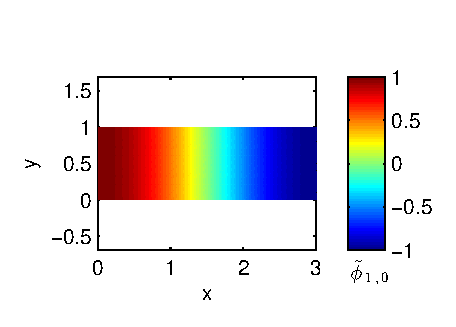
\includegraphics[width=\textwidth]{strip_cnts1}
\caption{}
\end{subfigure}
%
\begin{subfigure}{0.45\textwidth}
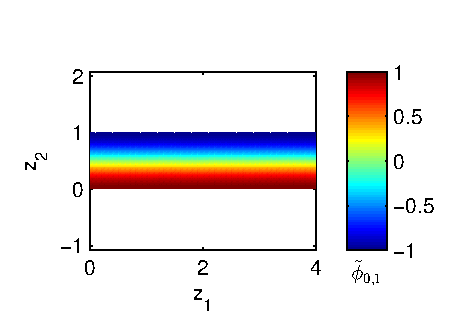
\includegraphics[width=\textwidth]{strip_cnts2}
\caption{}
\end{subfigure}
\caption{Two-dimensional strip colored by the eigenfunction (a) $\tilde{\phi}_{1, 0} = \cos \left( \frac{\pi z_1}{L_1} \right)$, and (b) $\tilde{\phi}_{0, 1} = \cos \left( \frac{\pi z_2}{L_2} \right)$ .}
\label{fig:strip_efuncs}
\end{figure}

We first consider the problem of parameterizing a continuous $d$-dimensional manifold $\mathcal{M}_d$ embedded in $\mathbb{R}^n$.
%
For linear hyperplanes,  the principal axes parameterize the manifold.
%
However, in the case when the manifold is curved, it is more difficult to define a set of coordinates. 

In recent years, it has been noted that eigenfunctions of the Laplace-Beltrami operator can be used to parameterize the manifold \cite{Belkin2003, coifman2005geometric, singer2008non}. 
%
To provide intuition as to why this is the case, consider a two-dimensional strip with edge lengths $L_1$ and $L_2$. 
%
The eigenvalues of the Laplace-Beltrami operator with Neumann boundary conditions are given by
\begin{equation} \label{eq:evals}
\tilde{\mu}_{k_1, k_2} = \left( \frac{k_1 \pi}{L_1} \right)^2 + \left( \frac{k_2 \pi}{L_2} \right)^2
\end{equation}
for $k_1, k_2 = 0, 1, 2, \dots$,
and the corresponding eigenfunctions are 
\begin{equation} \label{eq:efuncs}
\tilde{\phi}_{k_1, k_2} = \cos \left( \frac{k_1 \pi z_1}{L_1} \right) \cos \left( \frac{k_2 \pi z_2}{L_2} \right)
\end{equation}
where $z_1$ and $z_2$ denote the two coordinates of the rectangular domain \cite{singer2008non}. 
%
We note that the eigenfunctions $\tilde{\phi}_{1, 0} = \cos \left( \frac{\pi z_1}{L_1} \right)$ and $\tilde{\phi}_{0, 1} = \cos \left( \frac{\pi z_2}{L_2} \right)$ are one-to-one with the $z_1$ and $z_2$ coordinates, respectively, and therefore yield a parameterization of the underlying manifold (see Figure~\ref{fig:strip_efuncs}). 
%
Furthermore, the corresponding eigenvalues $\tilde{\mu}_{1,0}$ and $\tilde{\mu}_{0,1}$ provide a measure of $L_1$ versus $L_2$: as the ratio between $L_1$ and $L_2$ increases, the gap between $\tilde{\mu}_{1,0}$ and $\tilde{\mu}_{0,1}$ also increases (this will be discussed further in Section~\ref{sec:relative_lengths}).
%
Although these eigenfunctions can only be written analytically for very special cases, it has been observed empirically that the eigenfunctions often provide appropriate coordinates to parameterize more complex, nonlinear manifolds. 

 


\subsection{Discrete approximation of the Laplace-Beltrami operator: diffusion maps}

\begin{figure}[t]
\centering
\begin{subfigure}{0.45\textwidth}
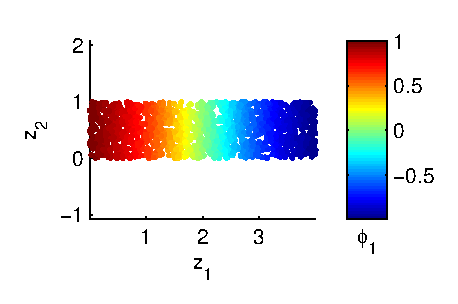
\includegraphics[width=\textwidth]{strip_discrete1}
\caption{}
\end{subfigure}
%
\begin{subfigure}{0.45\textwidth}
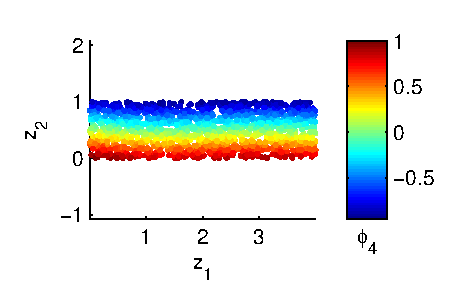
\includegraphics[width=\textwidth]{strip_discrete4}
\caption{}
\end{subfigure}

\begin{subfigure}{0.45\textwidth}
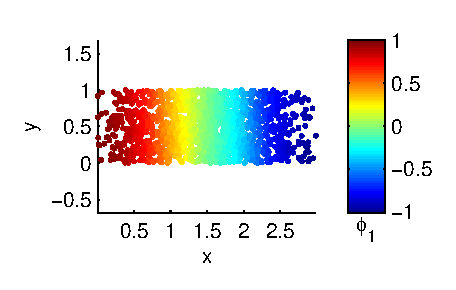
\includegraphics[width=\textwidth]{strip_nonuniform1}
\caption{}
\end{subfigure}
%
\begin{subfigure}{0.45\textwidth}
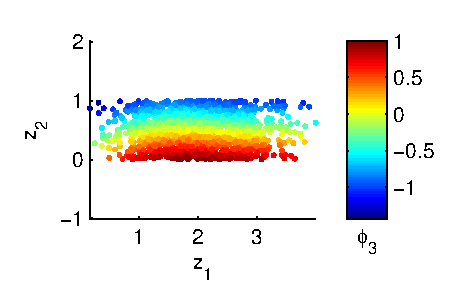
\includegraphics[width=\textwidth]{strip_nonuniform2}
\caption{}
\end{subfigure}
\caption{(a, b) Two-dimensional strip with uniform sampling colored by the (a) first, and (b) fourth (non-trivial) eigenvector from diffusion maps. (c, d) Two-dimensional strip with data sampled from a Gaussian distribution in $z_1$ and sampled uniformly in $z_2$, colored by the (c) first, and (d) third (non-trivial) eigenvector from diffusion maps. Note that in both cases we uncover parameterizations which are one-to-one with $z_1$ and $z_2$. }
\label{fig:strip_evecs}
\end{figure}

In most applications, we are not given a description of the continuous manifold. 
%
Instead, we are given data {\em sampled} from the underlying manifold, and we would like to uncover a parameterization of the data.
%
We will do this by constructing a matrix which approximates the Laplace-Beltrami operator with Neumann boundary conditions (TODO: is it explicit in the construction?). 
%
The eigenvectors of this matrix then approximate the eigenfunctions of this operator \cite{...}.

Assume we are given $m$ observations $z(1), \dots, z(m) \in \mathcal{M}_d$. 
%
We first construct the matrix $W \in \mathbb{R}^{m \times m}$, with
\begin{equation} \label{eq:W}
W_{ij} = \exp \left( -\frac{\|z(i) - z(j) \|^2}{\epsilon^2} \right), \ i,j=1,\ldots,m,
\end{equation}
where $\| \cdot \|$ denotes the appropriate norm for the observations, and $\epsilon$ is a characteristic distance between the observations. 
%
$\epsilon$ can be chosen using several heuristics \cite{coifman2008graph, rohrdanz2011determination}; we often take $\epsilon$ to be the median of the pairwise distances between the data points.
%
We then construct the diagonal matrix $D \in \mathbb{R}^{m \times m}$, with $D_{ii} = \sum_j W_{ij}$, and the matrix $A  = D^{-1} W.$
%
In the limit of infinite data uniformly sampled from $\mathcal{M}_d$ ($m \rightarrow \infty$ and $\epsilon \rightarrow 0$ with the appropriate rate), the matrix $I-A$ approaches the Laplace-Beltrami operator on the manifold $\mathcal{M}_d$ \cite{coifman2006geometric}. 
%
Therefore, the eigenvectors $\phi_0, \phi_1, \dots, \phi_{m-1}$ of $A$ approximate the eigenfunctions of the Laplace-Beltrami operator (with Neumann boundary conditions) on $\mathcal{M}_d$,
and the eigenvalues $\mu_0, \mu_1, \dots, \mu_{m-1}$ of $A$ are related to the eigenvalues of the continuous operator by 
\begin{equation} \label{eq:evals_relationship}
\mu_k = \exp \left( -\frac{\epsilon^2}{4} \tilde{\mu}_{k_1, k_2}  \right).
\end{equation}
%
As discussed previously, the eigenfunctions provide a parameterization of the manifold, such that $\phi_{j}(i)$ yields the $j^{th}$ embedding coordinate for $z(i)$.
%
We order the eigenvectors such that $|\mu_0| \ge |\mu_1| \ge \dots \ge |\mu_{m-1}|$, and if the data do lie on a low-dimensional manifold, we only need to retain a few of the leading eigenvectors to adequately describe the data.
%
Because the matrix $A$ is row-stochastic ($\sum_j A_{ij} = 1$),  $\mu_0 = 1$ and $\phi_0$ is a trivial constant vector which is not used as an embedding coordinate.

However, the data need not be sampled uniformly from the underlying manifold.
%
If the data $z(1), \dots, z(m)$ are sampled from $\mathcal{M}_d$ with some density $q$, then the matrix $I-A$ approximates the Fokker-Planck operator, 
\begin{equation}
(I-A) \phi \rightarrow \nabla^2 \phi - \nabla U \cdot \nabla \phi, 
\end{equation}
where $U = -2 \log q$. 
%
Alternatively, one can factor out the density effects in the diffusion maps matrix.
%
Given data $z(1), \dots, z(m) \in \mathcal{M}_d$, we construct the matrix
%
\begin{equation}
\tilde{W} = D^{-1} W D^{-1}.
\end{equation}
%
Pre- and post-multiplication by $D^{-1}$ removes any density effects from $W$. 
%
We then construct the diagonal matrix $\tilde{D} \in \mathbb{R}^{m \times m}$, with $\tilde{D}_{ii} = \sum_j \tilde{W}_{ij}$, and the matrix $\tilde{A}  = \tilde{D}^{-1} \tilde{W}.$
%
The matrix $\tilde{A}$ is comparable to the matrix $A$, but with sampling density effects removed, such that $I-\tilde{A}$ approaches the Laplace-Beltrami operator even if the data is nonuniformly sampled from the underlying manifold \cite{coifman2005geometric}. 

Figure~\ref{fig:strip_evecs} shows data sampled from a strip, colored by diffusion maps eigenvectors. 
%
In cases of both uniform and nonuniform sampling, the eigenvectors are one-to-one with $z_1$ and $z_2$, and thus parameterize the manifold. 
%
Although we have considered a very simple example for illustrative purposes, common practice is to use these tools for high-dimensional, nonlinear data sets.




\section{Identifying the Informative Eigenvectors }



In diffusion maps, we order the eigenvectors by the magnitude of the corresponding eigenvalues, in the hopes that the leading eigenvectors provide us with a parameterization of the underlying manifold.
%
However, often some eigenvectors are higher harmonics of previous eigenvectors and do not describe new directions in the data set \cite{gerber2007robust}.
%
Again, for illustrative purposes, we consider the case where $\mathcal{M}_d$ is a $2$-dimensional rectangular domain with edge lengths $L_1  > L_2$. 
%
We recall that the eigenfunctions $\tilde{\phi}_{1,0} = \cos \left( \frac {\pi z_1}{L_1} \right)$ and  $\tilde{\phi}_{0,1} = \cos \left( \frac {\pi z_2}{L_2} \right)$ provide embedding coordinates for the manifold $\mathcal{M}_d$. 
%
However, these two eigenvectors $\tilde{\phi}_{1, 0}$ and $\tilde{\phi}_{0, 1}$ are not guaranteed to correspond to the two smallest (non-trivial) eigenvalues (the largest eigenvalue will always be $\tilde{\mu}_{0,0} = 1$ and correspond to a constant eigenfunction; these eigenvalues are related to the diffusion maps eigenvalues $\mu_k$ via \eqref{eq:evals_relationship}). 
%
In fact, if $L_1 > 2 L_2$, then $\tilde{\mu}_{2, 0} < \tilde{\mu}_{0, 1}$, and so the second (non-trivial) eigenvector (when the eigenvectors are ordered by their corresponding eigenvalues) will be a repeated eigendirection of the first and still parameterize $z_1$ (see Figure~\ref{fig:strip_harmonics}).
%
We therefore require a methodology to automatically detect which eigenvectors are harmonics of each other. 
%
Utilizing only the diffusion maps eigenvectors which correspond to modes which are {\em not} higher harmonics yields the most parsimonious representation of the data.
%
We will show how we can automatically detect these modes to obtain a meaningful representation of the data.
%
Furthermore, the corresponding eigenvalues provide us with a measure of the relative lengths of the data set along the principal directions. 


\subsection{Algorithm: local linear regression}

\begin{figure}[t]
\centering
\begin{subfigure}{0.45\textwidth}
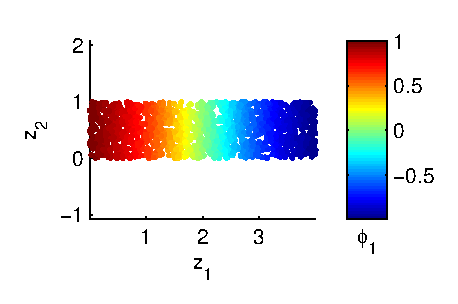
\includegraphics[width=\textwidth]{strip_discrete1}
\end{subfigure}
%
\begin{subfigure}{0.45\textwidth}
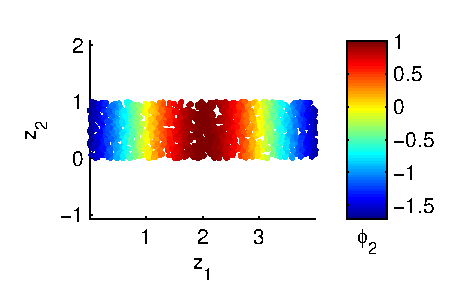
\includegraphics[width=\textwidth]{strip_discrete2}
\end{subfigure}

\begin{subfigure}{0.45\textwidth}
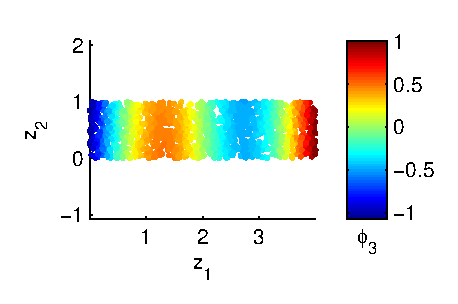
\includegraphics[width=\textwidth]{strip_discrete3}
\end{subfigure}
%
\begin{subfigure}{0.45\textwidth}
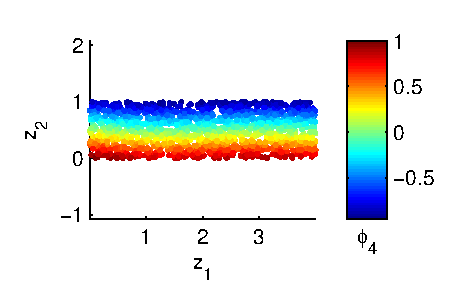
\includegraphics[width=\textwidth]{strip_discrete4}
\end{subfigure}
\caption{ Two-dimensional strip with uniform sampling colored by the first four (non-trivial) eigenvectors from diffusion maps. Note that the first and fourth eigenvectors are one-to-one with $z_1$ and $z_2$, respectively. However, the second and third eigenvectors are higher harmonics of the first eigenvector and do not capture any additional structure within the data set. }
\label{fig:strip_harmonics}
\end{figure}


Given the eigenvectors $\phi_1, \phi_2, \dots, \phi_{n-1} \in \mathbb{R}^m$, we would like to automatically deduce which ones capture new directions in the data, and which ones are merely repeated eigendirections. 
%
This problem was addressed previously in \cite{...} by performing successive iterations of diffusion maps, interspersed with advection along the first principal direction at each iteration. 
%
However, both the advection procedure and the successive eigendecompositions are very expensive and intractable for larger data set. 
%
Here, we propose an alternative approach to address the problem of repeated eigendirections. 
%
We will attempt to fit a function $f(\phi_1, \dots, \phi_{k-1})$ to $\phi_{k}$. 
%
If the resulting fit is accurate, then $\phi_{k}$ is most likely a harmonic of $\phi_1, \dots, \phi_{k-1}$. 
%
We will use a local linear function 
\begin{equation}
\phi_k \approx \alpha( \Phi_{k-1}) + \beta(\Phi_{k-1})^T \Phi_{k-1}
\end{equation}
%
as our functional approximation, where 
%
$\Phi_{k-1} = \begin{bmatrix} \phi_1 \\ \vdots \\ \phi_{k-1} \end{bmatrix}$
and $\beta \in \mathbb{R}^{k-1}$. 
%
The coefficients $\alpha$ and $\beta$ are functions of $\Phi_{k-1}$ because we use a {\em local} linear fit, and so the coefficients change as a function of the domain. 

At each point $\Phi_{k-1}(i)$, we approximate $\phi_k(i)$ by fitting a local linear function using the remaining $m-1$ data points. 
%
We solve the following optimization problem 
\begin{equation} \label{eq:opt_problem}
\hat{\alpha}_k (i) , \hat{\beta}_k(i)  = \argmin_{\alpha, \beta} \sum_{j \ne i} K(\Phi_{k-1}(i), \Phi_{k-1}(j)) \left( \phi_{k}(j) - (\alpha + \beta^T \Phi_{k-1}(j)) \right)^2.
\end{equation}
%
where $K$ is a kernel weighting function.
%
We will use a Gaussian kernel, 
%
\begin{equation}
K(\Phi_{k-1}(i), \Phi_{k-1}(j))  = \exp \left( - \frac{\|\Phi_{k-1}(i) - \Phi_{k-1} (j) \|^2}{\epsilon_{reg}^2} \right),
\end{equation}
%
where $\epsilon_{reg}$ is the kernel scale. 
%
We typically take $\epsilon_{reg} = M / 3$, where $M$ is the median of the pairwise distances between $\Phi_{k-1}(i)$, as we empirically found this choice to yield good results. 
%
We then define the normalized leave-one-out cross-validation error for this local linear fit as
\begin{equation} \label{eq:cv_error}
r_{k} = \sqrt{ \frac{\sum_{i=1}^n \left( \phi_{k} (i) - (\hat{\alpha}_k(i) + \hat{\beta}_k(i)^T \Phi_{k-1}(i))  \right)^2} {\sum_{i=1}^n  \left( \phi_{k} (i) \right)^2 }}
\end{equation}
%
Note that a small value of $r_k$ implies that $\phi_{k}$ can be accurately approximated from $\phi_1, \dots, \phi_{k-1}$, and is therefore a harmonic of a previous mode.
%
Conversely, a large value of $r_{k}$ indicates that $\phi_{k}$ parameterizes a new direction in the data.
%
Because $r_{k} \approx 1$ if $\phi_{k}$ parameterizes a new direction, we choose to define $r_1 = 1$.

\eqref{eq:cv_error} can easily be computed \cite{wasserman2006all}.
%
We begin by computing the matrix
\begin{equation}
X_{k-1}(i) = \begin{bmatrix}
1 & \phi_1(1) - \phi_1(i) & \dots & \phi_{k-1}(1)- \phi_{k-1}(i) \\
1 & \phi_1(2) - \phi_1(i) & \dots & \phi_{k-1}(2)- \phi_{k-1}(i) \\
\vdots & \vdots & \ddots & \vdots \\
1 & \phi_1(m) - \phi_1(i) & \dots & \phi_{k-1}(m)- \phi_{k-1}(i) 
\end{bmatrix}
\end{equation}
%
and the matrix 
\begin{equation}
W_{k-1}(i) = diag \left( K(\Phi_{k-1}(i), \Phi_{k-1}(1)), \dots, K(\Phi_{k-1}(i), \Phi_{k-1}(m)) \right).
\end{equation}
%
We then calculate the smoothing matrix $L_{k-1} \in \mathbb{R}^{m \times m}$, where 
\begin{equation}
L_{k-1} =
\begin{bmatrix}
e_1^T \left( X_{k-1}^T(1) W_{k-1}(1) X_{k-1}(1) \right) ^{-1} X_{k-1}^T(1) W_{k-1}(1) \\
e_1^T \left( X_{k-1}^T(2) W_{k-1}(2) X_{k-1}(2) \right) ^{-1} X_{k-1}^T(2) W_{k-1}(2) \\
\vdots \\
e_1^T \left( X_{k-1}^T(m) W_{k-1}(m) X_{k-1}(m) \right) ^{-1} X_{k-1}^T(m) W_{k-1}(m) \\
\end{bmatrix},
\end{equation}
%
where $e_1^T = (1, 0, \dots, 0)$. 
%
We can then write
%
\begin{equation} 
r_{k} = \sqrt{ \frac{\sum_{i=1}^n \left( \frac{ \phi_{k} (i) - \sum_{j=1}^m L_{k-1}(i,j) \phi_{k}(j) }{1-L_{k-1}(i,i)} \right)^2} {\sum_{i=1}^n  \left( \phi_{k} (i) \right)^2 }} .
\end{equation}

\subsection{Calculating the relative lengths of the manifold} \label{sec:relative_lengths}

Once we have determined which eigenvectors parameterize independent directions along the manifold, we can use the corresponding eigenvalues to calculate the relative lengths along these directions. 
%
Let $\mu_{i_1}, \mu_{i_2}, \dots$ denote the eigenvalues which correspond to eigenvectors which are {\em not} higher harmonics (i.e., those eigenvectors where $r_{i_j}$ is large). 
%
From \eqref{eq:evals} and \eqref{eq:evals_relationship}, we propose to approximate the relative lengths along the manifold by
\begin{equation} \label{eq:est_lengths}
L_j \propto \frac{1}{\sqrt{-\log \mu_{i_j}}}
\end{equation}
where $L_1, L_2, \dots$ are the relative lengths along the principal directions of the manifold. 
%
We can use this measure to determine how many components are required to retain most of the information within the data set: if $L_j$ is small, then this component can be disregarded (TODO: define small). 


\subsection{Illustrative examples} \label{sec:illustrative_examples}

We will demonstrate the local linear regression algorithm for identifying informative eigenvectors on three synthetic data sets. 
%
The first data set is a two-dimensional strip where the eigenvalues and eigenvectors are known analytically.
%
The second and third data sets are nonlinear manifolds which demonstrate the flexibility of our approach. 

\subsubsection{Strip}

\begin{figure}[t]
\centering
\begin{subfigure}{0.3\textwidth}
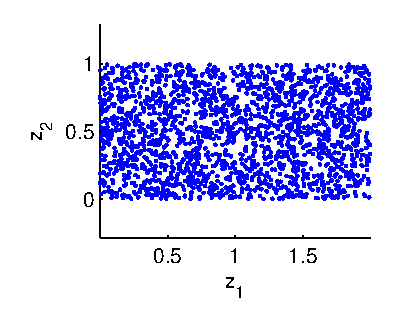
\includegraphics[height=2.5cm]{strip_data_L2}
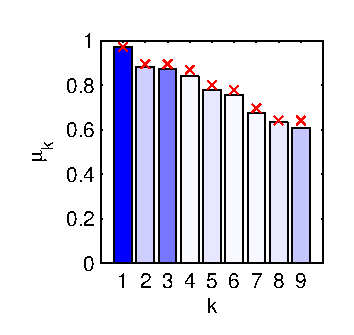
\includegraphics[height=3cm]{strip_spectrum_L2}
\caption{}
\end{subfigure}
%
\hfill
%
\begin{subfigure}{0.3\textwidth}
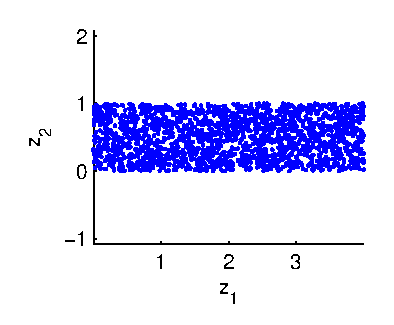
\includegraphics[height=2.5cm]{strip_data_L4}
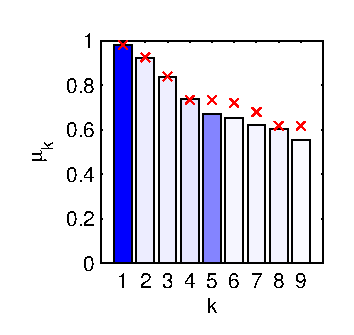
\includegraphics[height=3cm]{strip_spectrum_L4}
\caption{}
\end{subfigure}
%
\hfill
%
\begin{subfigure}{0.35\textwidth}
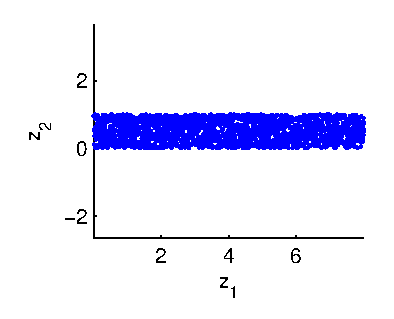
\includegraphics[height=2.5cm]{strip_data_L8}
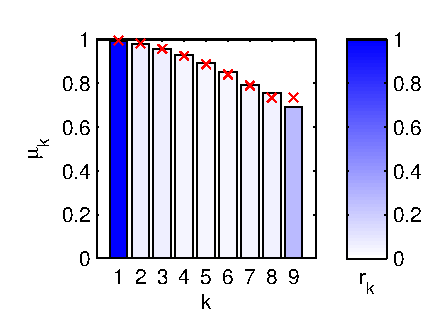
\includegraphics[height=3cm]{strip_spectrum_L8}
\caption{}
\end{subfigure}
%
\caption{Data sets (top) and eigenvalue spectra (bottom) for strips with (a) $L_1 = 2$, $L_2 = 1$, (b) $L_1 = 4$, $L_2 = 1$, (c) $L_1 = 8$, $L_2 = 1$. The empirical eigenvalues are plotted in blue, and the analytical eigenvalues are plotted in red. From the eigenvalues which are identified as important/non-harmonics, the estimated length ratio is (a) 2.0, (b) 4.4, (c) 8.8.  }
\label{fig:strip_compare_analytic}
\end{figure}

Our first illustrative example consists of three different two-dimensional strip data sets. 
%
Each data set contains $m=1500$ data points uniformly sampled from the strip. 
%
Figure~\ref{fig:strip_compare_analytic} shows the data sets and corresponding eigenspectra.
%
The eigenvalues are colored by the leave-one-out cross-validation error as defined in \eqref{eq:cv_error}; a small value of $r_k$ indicate that the corresponding eigenvector is a harmonic of previous eigenvectors, while a large value of $r_k$ indicates that the corresponding eigenvector describes a new direction in the data. 
%
As expected, the gap between the two meaningful eigenvalues increases as the strip becomes narrower. 
%
The diffusion maps eigenvalues are consistent with the known analytic eigenvalues of the Laplacian (see \eqref{eq:evals} and \eqref{eq:evals_relationship}), and using \eqref{eq:est_lengths}, we can accurately estimate the relative lengths of the two principal directions in each data set. 


\subsubsection{Swiss roll}

\begin{figure}[!th]
%
\begin{subfigure}{0.45\textwidth}
\centering
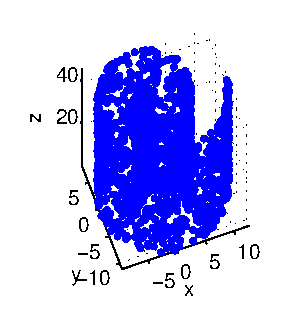
\includegraphics[height=1.25in]{swissroll1}
\caption{}
\end{subfigure}
\hfill
\begin{subfigure}{0.45\textwidth}
\centering
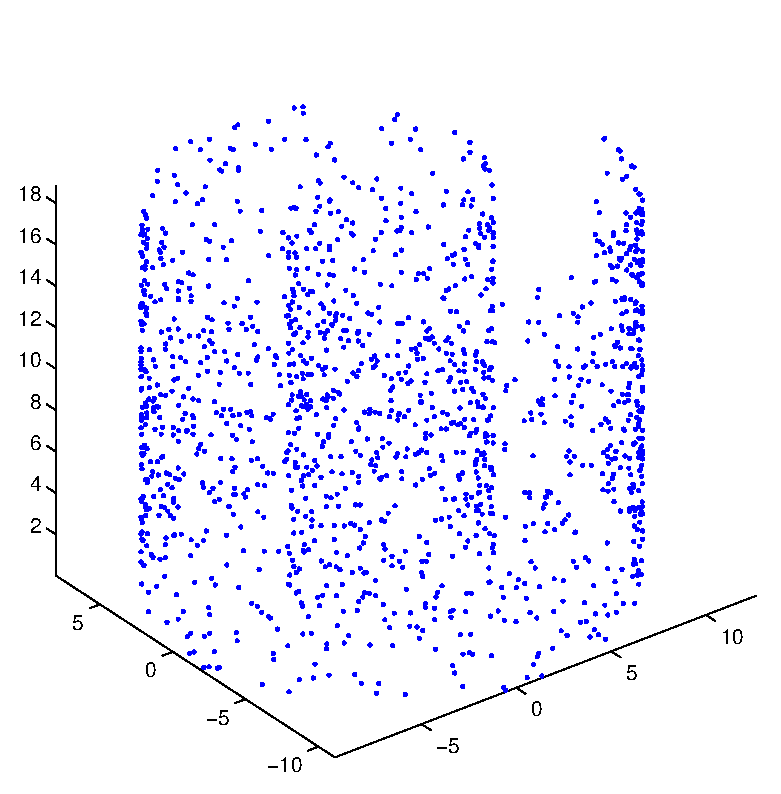
\includegraphics[height=1.25in]{swissroll2}
\caption{}
\end{subfigure}
\hfill
\begin{subfigure}{0.45\textwidth}
\centering
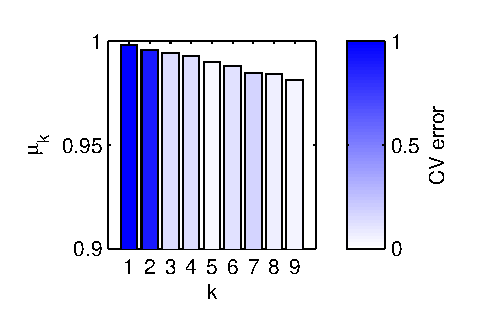
\includegraphics[height=1.25in]{swissroll1_evals}
\caption{}
\end{subfigure}
\hfill
\begin{subfigure}{0.45\textwidth}
\centering
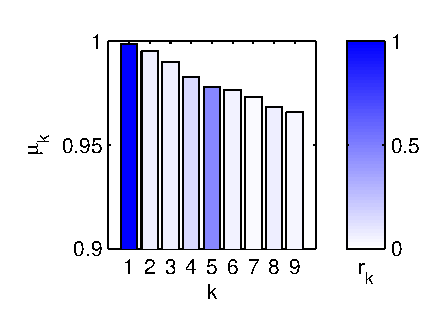
\includegraphics[height=1.25in]{swissroll2_evals}
\caption{}
\end{subfigure}
\hfill
\begin{subfigure}{0.45\textwidth}
\centering
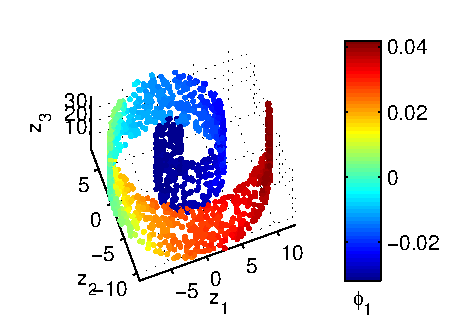
\includegraphics[height=1.25in]{swissroll1_color1} 
\caption{}
\end{subfigure}
\hfill
\begin{subfigure}{0.45\textwidth}
\centering
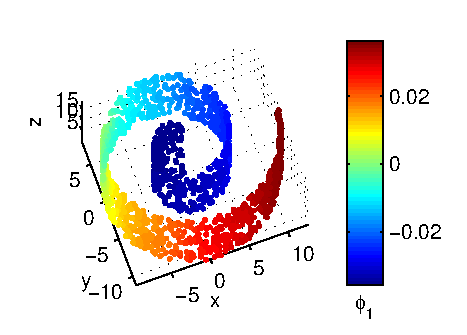
\includegraphics[height=1.25in]{swissroll2_color1}
\caption{}
\end{subfigure}
\hfill
\begin{subfigure}{0.45\textwidth}
\centering
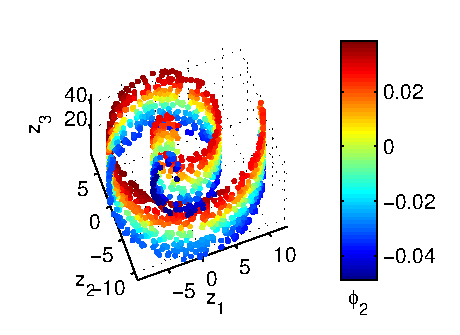
\includegraphics[height=1.25in]{swissroll1_color2}
\caption{}
\end{subfigure}
\hfill
\begin{subfigure}{0.45\textwidth}
\centering
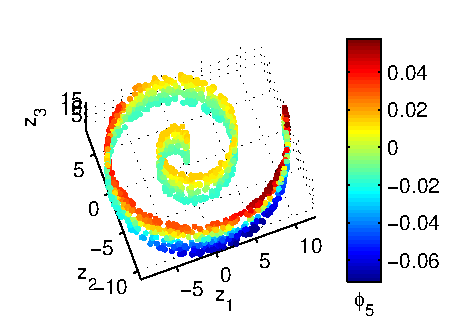
\includegraphics[height=1.25in]{swissroll2_color2}
\caption{}
\end{subfigure}
%
\caption{Swiss roll example. (a) Data set 1; $h= 40$. (b) Data set 2; $h = 20$. (c) Diffusion maps eigenvalue spectrum for data set 1. (d) Diffusion maps eigenvalue spectrum for data set 2. (e) Data set 1, colored by the first diffusion maps eigenvector. (f) Data set 2, colored by the first diffusion maps eigenvector. (g) Data set 1, colored by the second diffusion maps eigenvector which is not a harmonic of the first. (h) Data set 2, colored by the second diffusion maps eigenvector which is not a harmonic of the first. } 
\label{fig:swiss_rolls}	
\end{figure}

Our second illustrative example consists of two different swiss roll data sets.
%
The data are
\begin{equation}
\begin{aligned}
z_1 =& \theta \cos \theta \\
z_2 =& \theta \sin \theta \\
z_3 =& h t
\end{aligned}
\end{equation}
%
such that $z_1, z_2$ are uniformly sampled along the arclength of the spiral, and $t \sim Unif(0,1)$. 
%
The height of the first swiss roll is $h = 40$, while the height of the second is $h = 20$. 
%
Each data set consists of $m=1500$ points, shown shown in Figure~\ref{fig:swiss_rolls}(a)~and~(b).
%
We expect to recover the eigenvector which parameterizes the height farther down in the spectrum for the second data set relative to the first, as this second data set is shorter.

Figure~\ref{fig:swiss_rolls}~(c)~and~(d) shows the diffusion maps eigenvalue spectra for the two data sets.
%
Again, the bars are colored by the leave-one-out cross-validation error, where a small value of $r_k$ indicates that the corresponding eigenvector is a harmonic of previous eigenvectors. 
%
From these plots, one can conclude that the first two eigenvectors $\phi_1$ and $\phi_2$ parameterize the first data set, while $\phi_1$ and $\phi_5$ parameterize the second. 
%
Figure~\ref{fig:swiss_rolls}~(e--h) shows the two data sets, colored by the two ``important'' eigenvectors. 
%
As expected, these eigenvectors parameterize the arc length along the spiral, and the height of the swiss roll. 

\subsubsection{Torus}

\begin{figure}[t]
%
\begin{subfigure}{0.3\textwidth}
\centering
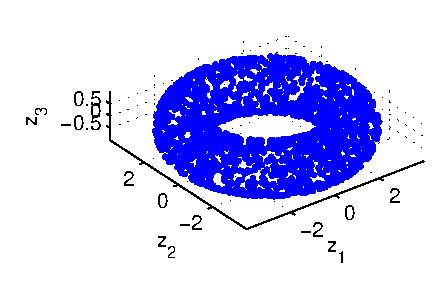
\includegraphics[height=0.75in]{torus1}
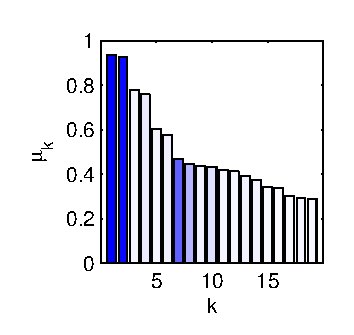
\includegraphics[height=1in]{torus1_evals}
\caption{}
\end{subfigure}
%
\hfill
%
\begin{subfigure}{0.32\textwidth}
\centering
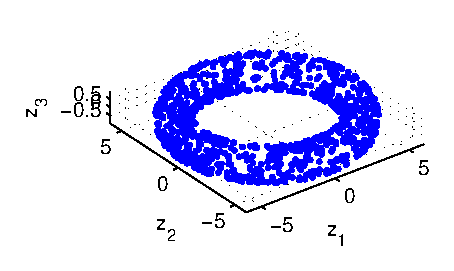
\includegraphics[height=0.75in]{torus2}
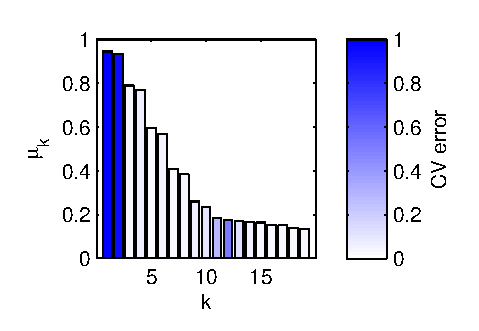
\includegraphics[height=1in]{torus2_evals}
\caption{}
\end{subfigure}
%
\hfill
%
\begin{subfigure}{0.35\textwidth}
\centering
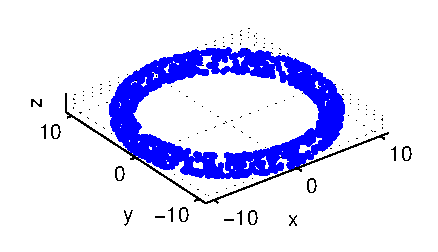
\includegraphics[height=0.75in]{torus3}
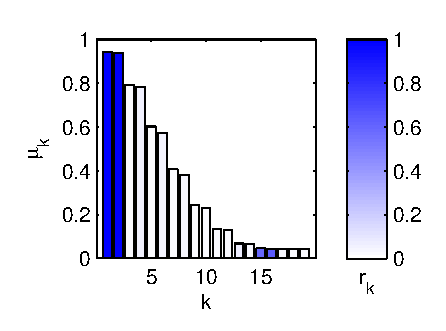
\includegraphics[height=1in]{torus3_evals}
\caption{}
\end{subfigure}
%
\hfill
%
\caption{Torus data sets (left) and corresponding diffusion maps eigenvalues (right). (a) $r_1 = 3$, $r_2 = 1$. (b) $r_1 = 5$, $r_2 = 1$. (c) $r_1 = 10$, $r_2 = 1$. In all three data sets, the first two eigenvalues/eigenvectors correspond to $\sin \theta_1$ and $\cos \theta_1$. The second pair of non-harmonic eigenvectors (corresponding to $\sin \theta_2$ and $\cos \theta_2$) are captured by components 7 and 8, 11 and 12, and 15 and 16, respectively.}
%
\label{fig:torus}
%
\end{figure}

For the third example, we consider a torus defined by
%
\begin{equation}
\begin{aligned}
z_1 =& (r_1 + r_2 \cos \theta_2 ) \cos \theta_1 \\
z_2 =& (r_1 + r_2 \cos \theta_2 ) \sin \theta_1 \\
z_3 =& r_2 \sin \theta_2
\end{aligned}
\end{equation}
%
where $r_1 > r_2$ are the outer and inner radii, respectively, and $\theta_1, \theta_2 \sim Unif(0, 2 \pi)$. 
%
Changing the ratio of $r_1$ to $r_2$ changes the ratio of the eigenvalues corresponding to non-harmonic eigenvectors. 

We expect to obtain two eigenfunctions ($\sin \theta_1$ and $\cos \theta_1$) which parmeterize the outer circle, and two eigenfunctions ($\sin \theta_2$ and $\cos \theta_2$) which parameterize the inner circle. 
%
However, the number of harmonics which fall between the two pairs of descriptive eigenfunctions depends on the ratio of the two radii. 

Figure~\ref{fig:torus} shows the diffusion maps eigenspectra for three different torii, again colored by the leave-one-out cross-validation error. 
%
Clearly, as the torus becomes thinner, the second pair of relevant eigenfunctions (corresponding to $\sin \theta_2$ and $\cos \theta_2$) moves farther down in the spectrum. 

\section{Chemotaxis: A Case Study}

Our main motivation for factoring out the harmonics in diffusion maps is to facilitate the analysis of complex data sets where the underlying structure is not readily apparent. 
%
In data from complex dynamical systems, noisy microscopic behavior often gives rise to cohernt macroscopic dynamics. 
%
%Although on the microscale the system consists of many stochastic and noisy particles, it exhibits coherent dynamics on the macroscale which are governed by only a few parameters.
%
In general, this mapping from microscale to macroscale is not always obvious.
%
We will show how we can use diffusion maps to extract a parameterization of data collected at the microscale which is consistent with the macroscopic behavior, without any {\em a priori} knowledge of the appropriate microscopic or macroscopic model.
%
Furthermore, determining the {\em true} dimensionality of such a parameterization by factoring out higher harmonics in the diffusion maps analysis uncovers the requisite dimensionality of a reduced model which captures the relevant macroscopic behavior. 
%
Knowing appropriate macroscopic variables and the true dimensionality can help inform modeling efforts and aid in the writing of accurate macroscale models.



%For example, fluid flow, which can be described via the position and velocity of every fluid particle, is modeled at the macroscale using the Navier-Stokes equations.
%

%In this letter, we will demonstrate how this goal can be achieved through a data-driven method based on geometric analysis and manifold learning. 
%
%Specifically, we aim to emphasize two particular aspects of manifold learning from a dynamical systems' point of view: (a) choosing the appropriate observers, especially in presence of stochastic dynamics, and (b) selecting an appropriate metric for comparison \cite{mallat2012group}. 
%
%We will show that both are essential for data-driven algorithms to successfully uncover the underlying system dynamics. 

Our model problem comes from studies of cellular chemotaxis \cite{othmer2000diffusion}, where biological cells work together and exhibit coherent macroscopic dynamics regulated by extracellular sensed signals in order to accomplish tasks such as finding food or navigating away from toxins.
%
Several microscopic models have been proposed to describe chemotaxis dynamics \cite{othmer1988models, codling2008random}.
%
We will analyze one such model described by a one-dimensional velocity jump process \cite{othmer2000diffusion}.
%
In this model, each cell is initialized with a position and a velocity on a line, and the dynamics of each cell are governed by a stochastic process.
%
At random times, a cell will ``turn around'' and switch the direction of its velocity (this turning is controlled by extracellular signals). 
%
%We will analyze the dynamics of collections of such cells/particles. 

%In this example, the macroscopic dynamics of the group of cells vary depending on the value of a single system parameter.
%
%We will demonstrate how we can use diffusion maps \cite{coifman2005geometric}, a manifold learning technique, to {\em automatically} detect changes in the system's macroscopic dynamics from microscale data.
%
%This case study exhibits several key points which allow us to demonstrate the strength of our diffusion maps approach.
%
%First, this system has random microscopic behavior with smooth macroscopic dynamics governed by a single parameter which determines the regime/mode of the system. 
%
%Second, it consists of an ensemble of individual stochastic particles which must be described using the appropriate observers.
%
%Third, it has an analytic macroscopic description, which serves as a ground truth and will allow us to verify our results which are obtained in an unsupervised manner.
This specific example has an analytic macroscopic description in which the macroscopic dynamics of the group of cells vary depending on the value of a single system parameter.
%
This model serves as a ground truth and will allow us to verify our results which are obtained in an unsupervised manner.
%
We will show that manifold learning algorithms based on statistical observers and with the appropriate affinity metric between pairs of observations uncovers a parameterization of the microscopic data which is consistent with the macroscopic model.
%
Furthermore, these data-driven methods allow us to detect changes in dynamical behavior resulting from changes in the system parameters. 

%The remainder of this letter is organized as follows. 
%
%We begin by describing the chemotaxis problem, the illustrative example used to demonstrate the methodologies.
%%
%We present the stochastic microscopic model, and use diffusion maps, a nonlinear dimensionality reduction technique, to analyze microscopic simulation results.
%%
%We show that the governing macroscopic variables can be recovered, provided that the appropriate observers and distance metric are used.
%%
%We then describe how, for this example, the microscopic model gives rise to a compact macroscopic description governed by a single parameter, and show that the diffusion maps results are consistent with this macroscopic description. 
%%
%Finally, we demonstrate that diffusion maps can also identify the relative importance of system variables in different parameter regimes, and detect changes in macroscopic dynamical behavior.

%\section{Problem formulation}

%\subsection{Chemotaxis ``story''} 


\subsection{Problem description}

The microscopic model consists of a collection of $N$ particles whose states are defined by their positions and velocities. 
%
Let $x_i(t)$ and $v_i(t)$ denote the position and velocity, respectively, of particle $i$ at time $t$.
%
The velocity of each particle is either $\pm s$, where $s$ is a (fixed) speed. 
%
We initialize the particles such that
\begin{equation}\label{eqn:system}
\begin{aligned}
x_i(0) & = 0 \\
\mathbb{P} \{ v_i(0) = +s \} & = p
\end{aligned}
\end{equation}
where $0 < p < 1$ is the probability of a particle initially moving to the right.
%
The velocity of each particle randomly switches between $\pm s$ following an (independent) Poisson process with rate $\lambda$.
%
We would like to note that we have chosen a very specific one-parameter family of initial conditions which lead to simple dynamics and straightforward illustration of our main points;
more complex initial conditions could easily be chosen. 

This particular example has a known analytic macroscopic equation that governs the overall system behavior.
%
For a large collection of particles ($N \rightarrow \infty$), the system can be described by the probability density of the particles.
%
Let $\rho(x, t)$ denote the probability density of the particles, and let $\rho^-(x, t)$ and $\rho^+(x, t)$ denote the densities of the particles moving towards the positive and negative axis directions, respectively.
%
It can be shown that, as $N \rightarrow \infty$, the densities obey the following set of partial differential equations (PDEs) \cite{othmer2000diffusion}:
\begin{equation} \label{eqn:coupled_pdes}
\begin{aligned}
\frac{\partial \rho^+}{\partial t} + s \frac{\partial \rho^+}{\partial x} & = -\lambda \rho^+ +\lambda \rho^- \\
\frac{\partial \rho^-}{\partial t} - s \frac{\partial \rho^-}{\partial x} & = \lambda \rho^+ -\lambda \rho^- 
\end{aligned}
\end{equation}
%
Alternatively, \eqref{eqn:coupled_pdes} can be rewritten as one, second--order PDE:
\begin{equation} \label{eq:second_order_pde}
\frac{\partial^2 \rho}{\partial t^2} + 2 \lambda \frac{\partial \rho}{\partial t} = s^2 \frac{\partial ^2 \rho}{\partial x^2}
\end{equation}
%
%We assume that $s^2/\lambda = D$ is constant, so that the dynamics of the probability density are governed by a {\em single} parameter $\lambda$.
%
From \eqref{eq:second_order_pde}, we see that, for fixed values of $\lambda$ and $s$, the macroscopic state of the system (the probability density of the particles) is a function of two independent variables: $p$, which controls the initial distribution of the particles, and $t$, the time. 
%
This implies that for fixed $\lambda$ and $s$, the {\em microscopic} data in a high-dimensional ambient space (e.g., the positions of all $N$ particles) should lie on a two-dimensional manifold parameterized by $p$ and $t$, 
and uncovering the low-dimensional structure of the microscopic data reveals this manifold.

We consider two asymptotic regimes of simulation.
%
When $\lambda \rightarrow 0$, the right-hand side of \eqref{eqn:coupled_pdes} tends to 0, and \eqref{eqn:coupled_pdes} becomes two uncoupled wave equations,
\begin{equation}
\begin{aligned}
\frac{\partial \rho^+}{\partial t} + s \frac{\partial \rho^+}{\partial x} & = 0 \\
\frac{\partial \rho^-}{\partial t} - s \frac{\partial \rho^-}{\partial x} & = 0.
\end{aligned}
\end{equation}
%alternatively, \eqref{eq:second_order_pde} becomes the second order wave equation,
%\begin{equation}
%\frac{\partial^2 \rho}{\partial t^2} = s^2 \frac{\partial ^2 \rho}{\partial x^2}.
%\end{equation}

%Dividing \eqref{eq:second_order_pde} by $\lambda > 0$ yields
%\[
%\frac{1}{\lambda} \frac{\partial^2 \rho}{\partial t^2} + 2 \frac{\partial \rho}{\partial t} = D \frac{\partial ^2 \rho}{\partial x^2}
%\]
When $\lambda \rightarrow \infty$, \eqref{eq:second_order_pde} approaches the heat equation,
\begin{equation}
2 \frac{\partial \rho}{\partial t} = D \frac{\partial ^2 \rho}{\partial x^2}.
\end{equation}
%
%Two variables determine the macroscopic state of the system: the initial distribution, which is controlled by a single parameter $p$, and the time, $t$.
%
The above analysis shows that the initial distribution of velocities of the particles (determined by $p$ in the microscopic simulations) plays a very different role depending on the value of $\lambda$.
%
When $\lambda \rightarrow 0$, the dynamics are described by two wave equations, and the initial distribution persists throughout the trajectory.
%
When $\lambda \rightarrow \infty$, the dynamics are described by one heat equation, and the initial conditions are insignificant -- the velocity distribution quickly equilibrates and we see purely diffusive behavior.
%
We therefore expect the observed dimensionality to change from two to one as a function of $\lambda$. 
%
For general dynamical systems, the governing macroscopic variables and asymptotic behavior may not be immediately obvious, and instead need to be inferred from the microscopic data.
%
We will demonstrate how we can use diffusion maps to parameterize the simulation data, as well as detect the effective dimensionality of the data.
%
%We expect the simulation data to lie on a low-dimensional manifold which is parameterized by the macroscopic variables.
%
%We use diffusion maps \cite{coifman2005geometric}, which is a manifold learning technique, to uncover such low-dimensional structure and to analyze the results of the microscopic chemotaxis simulations.
%
%Compared to principal components analysis (PCA) \cite{shlens2005tutorial}, a standard linear technique, diffusion maps provides a parameterization of data which lie on a low-dimensional, (possibly) {\em nonlinear} structure in a high-dimensional space.
%
%Diffusion maps is one of many recently introduced manifold learning techniques that could be used to analyzed this data \cite{roweis2000nonlinear, tenenbaum2000global, Belkin2003}.




\subsection{Observers and metrics}

In general, manifold learning techniques have two essential components.
%
One is the appropriate {\em observers} of the system. 
%
These observers should be informative as to the state of the system, as well as insensitive to noise in the system. 
%
Two is a {\em distance metric} between the observations that captures a notion of locality: observations which we perceive to be similar should have a small distance. 
%
%For this particular example, we will use histograms of the particle positions as the observations, and the EMD as the distance metric.


Appropriate observers can be constructed in several different ways. 
%
For simple data, such as the illustrative examples in Section~\ref{sec:illustrative_examples}, the observers are simply the data points themselves. 
%
However, for more complex data, the raw data may contain other sources of variability which are not meaningful to the system dynamics. 
%
For some examples, physical intuition and {\em a priori} knowledge can aid in constructing appropriate observers. 
%
For example, when looking at a protein, the observers may be the locations of the $\alpha$-carbons, as these backbone atoms are known to capture most of the relevant dynamics. 
%
Observers can also remove unimportant sources of variation; 
for example, the bispectrum \cite{zhao2014rotationally} and the scattering transform \cite{mallat2012group} are both invariant to rotations. 
%
Observers should also be robust to noise, which motivates the scattering transform \cite{mallat2012group} and histograms \cite{talmon2013empirical}.

After constructing appropriate observers, one must choose the appropriate metric for the diffusion maps calculation. 
%
The simplest option (used for the illustrative examples in Section~\ref{sec:illustrative_examples}) is to use the Euclidean distance, but this can often prove uninformative. 
%
For molecular simulation data, it is often appropriate to use the Euclidean distance {\em after} aligning configurations with respect to rotations, as global rotations of the entire molecule are not meaningful \cite{ferguson2010systematic}.
%
For dynamical systems which are obscured by large variance noise, the Mahalanobis distance often yields a more informative parameterization of the data \cite{talmon2013empirical}.
%
Another option is the Earth Mover's Distance, a multiscale distance metric which is stable and robust to noise \cite{rubner2000earth}.

For the chemotaxis example, we use histograms of the particle positions as observers \cite{talmon2013empirical}. 
%
Histograms are invariant to the indexing of the particles, while retaining the spatial locations of the particles.
%
Instead of the standard Euclidean distance, we use the earth mover's distance (EMD) \cite{rubner2000earth} as the metric between pairs of histograms. 
%
Conceptually, the EMD measures how much ``work'' it takes to transform one probability density into another.
%
It therefore not only considers where the densities are inconsistent, but also how far apart the inconsistencies are.
%
Although the brute-force computation of the EMD is computationally expensive, there has been a plethora of work in developing efficient algorithms for its computation \cite{Pele-eccv2008, Pele-iccv2009}.
%
For the special case of one-dimensional data, the EMD is equivalent to the $L_1$-norm between the cumulative distribution functions \cite{rubner2000perceptual}, which can be estimated from histograms as
\begin{equation}
\| z(i) - z(j) \|_{EMD} \approx \sum_{l=1}^{n} \left| \sum_{k=1}^l z_k(i) - \sum_{k=1}^l z_k(j) \right|
\end{equation}
where the histograms $z(i), z(j)$ are defined on equally-spaced bins in $\mathbb{R}$, and $z_k$ denotes the $k^{th}$ bin. 
%
We note that although histograms are not essential for using EMD, histograms make the computation feasible. 
%
The histograms are also robust to noise \cite{talmon2013empirical}. 

%\subsubsection{Constructing appropriate observers}
%
%\begin{itemize}
%\item Physical examples (e.g., $\alpha$-carbons for molecules)
%\item Amit's bispectrum
%\item Scattering transform
%\item Cite PNAS, stating that the histograms are good since they linearize any noise. 
%For the chemotaxis example, we use histograms of the particle positions as observers \cite{talmon2013empirical}. 
%%
%Histograms are invariant to the indexing of the particles, while retaining the spatial locations of the particles.
%\end{itemize}
%
%\subsubsection{Defining a meaningful metric}
%
%
%\begin{itemize}
%\item Euclidean (not good, especially for histograms)
%\item Mahalanobis (good, cite PNAS, since it noise robust)
%\item Here we use EMD since it is multiscale.
%%
%Instead of the standard Euclidean distance, we use the earth mover's distance (EMD) \cite{rubner2000earth} as the metric between pairs of histograms. 
%%
%Conceptually, the EMD measures how much ``work'' it takes to transform one probability density into another.
%%
%It therefore not only considers where the densities are inconsistent, but also how far apart the inconsistencies are.
%%
%Although the brute-force computation of the EMD is computationally expensive, there has been a plethora of work in developing efficient algorithms for its computation \cite{Pele-eccv2008, Pele-iccv2009}.
%%
%For the special case of one-dimensional data, the EMD is equivalent to the $L_1$-norm between the cumulative distribution functions \cite{rubner2000perceptual}, which can be estimated from histograms as
%\begin{equation}
%\| z(i) - z(j) \|_{EMD} \approx \sum_{l=1}^{n} \left| \sum_{k=1}^l z_k(i) - \sum_{k=1}^l z_k(j) \right|
%\end{equation}
%where the histograms $z(i), z(j)$ are defined on equally-spaced bins in $\mathbb{R}$, and $z_k$ denotes the $k^{th}$ bin. 
%%
%\item Emphasize stability and regularity issues.
%\end{itemize}






\subsection{Results}


\subsubsection{Using the appropriate metric}

\begin{figure}[t!]
\centering
\begin{subfigure}{5cm}
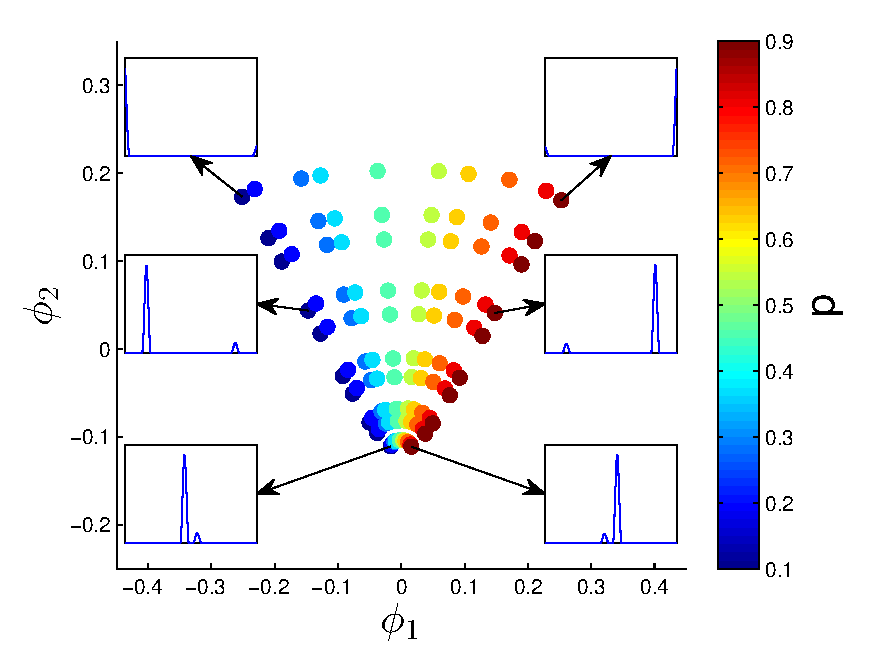
\includegraphics[width=\textwidth]{EMD_withhist_p_1}
\caption{}
\label{subfig:small_lambda_p}
\end{subfigure}
\begin{subfigure}{5cm}
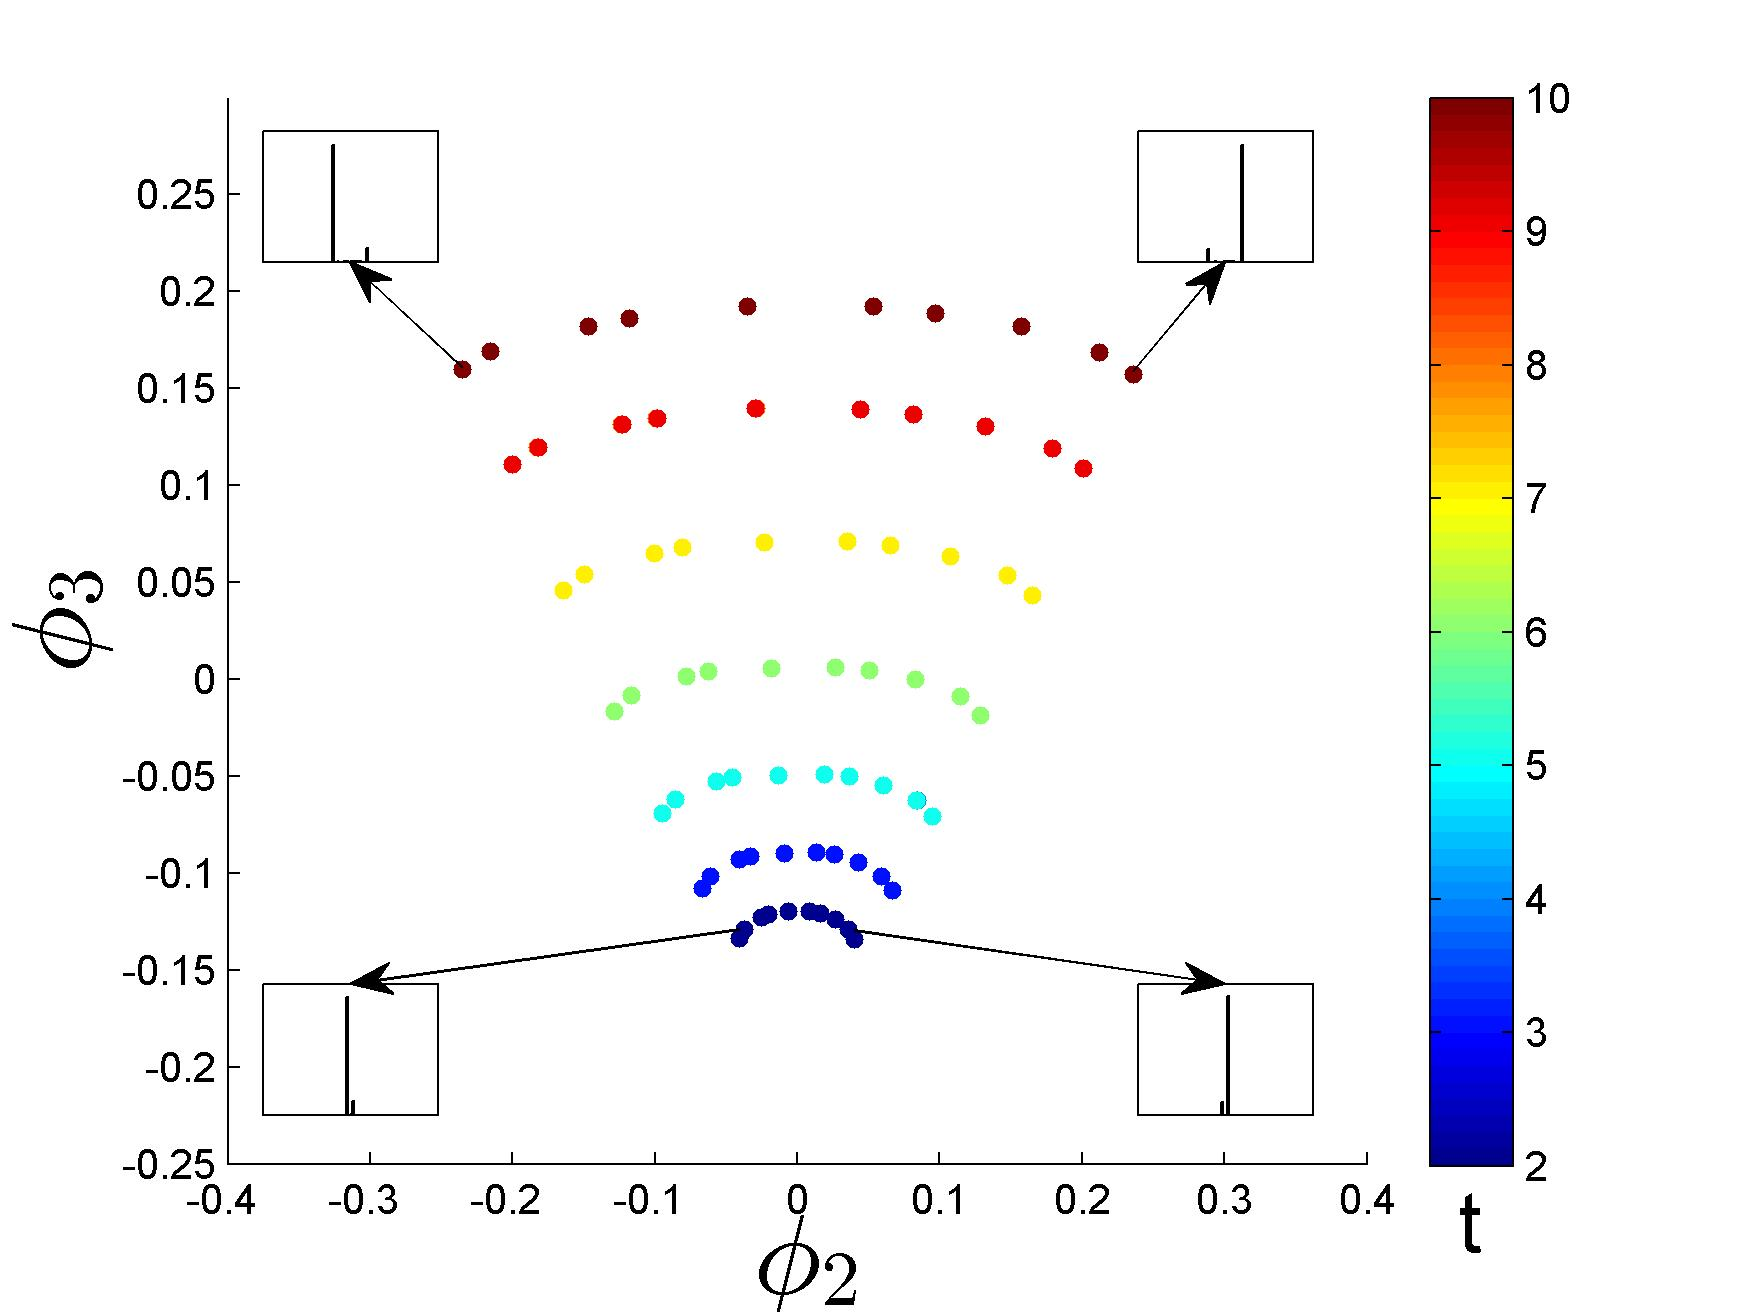
\includegraphics[width=\textwidth]{EMD_withhist_t_1}
\caption{}
\label{subfig:small_lambda_t}
\end{subfigure}
\begin{subfigure}{5cm}
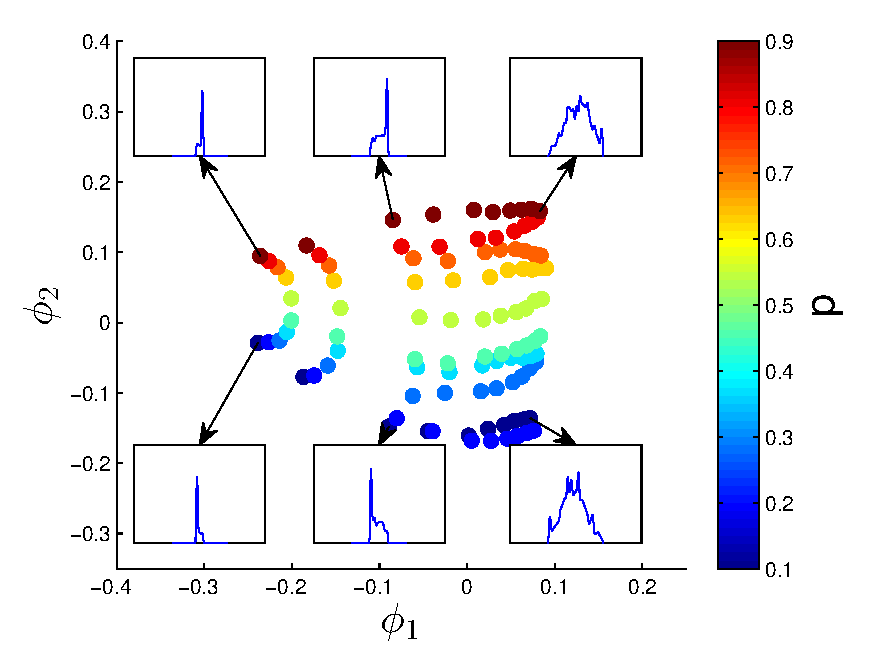
\includegraphics[width=\textwidth]{EMD_withhist_p_400}
\caption{}
\label{subfig:large_lambda_p}
\end{subfigure}
\begin{subfigure}{5cm}
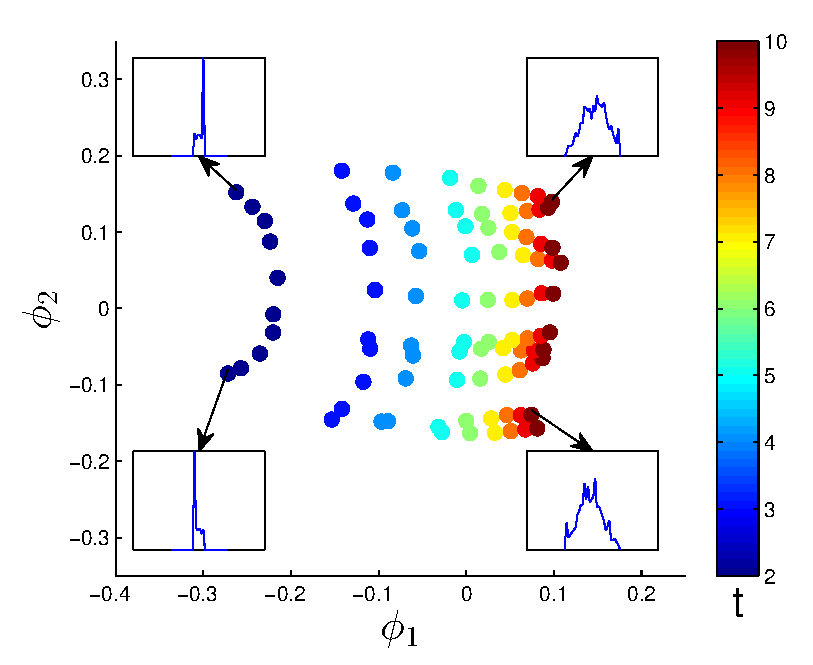
\includegraphics[width=\textwidth]{EMD_withhist_t_400}
\caption{}
\label{subfig:large_lambda_t}
\end{subfigure}
\caption{Diffusion maps embeddings computed from simulation data of the velocity jump process with (a,b) $\lambda=1$, $s=1$, and (c,d) $\lambda=400$, $s=20$.  For each set, we run many simulations, each with $N=1000$ particles.
%
We vary the initial conditions such that $0.1 \le p  \le 0.9$, and allow each simulation to evolve for $10$ time units.
%
We discard the initial portion of each simulation trajectory ($t < 1$), which corresponds to the initial relaxation of the system.
%
The observation $z(i) \in \mathbb{R}^n$ is the histogram of $x_1(i), x_2(i), \dots, x_N(i)$ into $n = 32$ bins.
%
The distances used in the diffusion maps kernel are the earth mover's distances between the histograms of particle positions. The data are colored by (a, c) $p$, the initial probability of a particle moving to the right, and (b, d) $t$, time. Representative histograms are shown for selected data points.}
\label{fig:dmaps_embed_emd}
\end{figure}


Figure~\ref{fig:dmaps_embed_emd} shows the results of analyzing two sets of chemotaxis simulations using diffusion maps. 
%
One set of simulations (Figures~\ref{subfig:small_lambda_p}~and~\ref{subfig:small_lambda_t}) is for a small value of $\lambda$, and the other set (Figures~\ref{subfig:large_lambda_p}~and~\ref{subfig:large_lambda_t}) is for a large value of $\lambda$. 
%
For both sets of simulations, the two macroscopic variables, $p$ and $t$, are well-correlated with the first two diffusion maps coordinates, $\phi_1$ and $\phi_2$. 
%
In both cases, $\phi_1$ is significantly more important than $\phi_2$, as indicated by the separation between the first two eigenvalues (for the small $\lambda$ case, $\mu_1 = 0.5138$, and $\mu_2 = 0.3943$, and for the large $\lambda$ case, $\mu_1 = 0.5543$, and $\mu_2 = 0.3807$).
%
$\phi_1$, the ``more important'' coordinate, is correlated with $p$ for the small $\lambda$ case (Figure~\ref{subfig:small_lambda_p}), and correlated with $t$ for the large $\lambda$ case (Figure~\ref{subfig:large_lambda_t}), indicating that the relative importance of $p$ and $t$ changes in the two simulations;
this is consistent with the analytic macroscopic description. 
%
Furthermore, in the small $\lambda$ regime (wave equation), shown in Figures \ref{subfig:small_lambda_p} and \ref{subfig:small_lambda_t}, the points corresponding to small times are more tightly clustered than the points corresponding to large times.
%
This is in agreement with the macroscopic model: at small times, the particles are more condensed around $x=0$, and it is more difficult to distinguish the particles moving to the left from the particles moving to the right. 
%
On the other hand, at large times, once the particles evolve from the origin, this separation is clear.  
%
For the large $\lambda$ case (heat equation), shown in Figures \ref{subfig:large_lambda_p} and \ref{subfig:large_lambda_t}, we observe that at small times, the initial distribution $p$ is well organized in the embedding in Figure \ref{subfig:large_lambda_p}, as the skew of the velocity distribution can be seen in the initial displacements.
%
On the other hand, for large times, we observe that the initial distribution $p$ is less organized in Figure \ref{subfig:large_lambda_p}, as the velocities have equilibrated and the initial distribution is less detectable in the particle density.
%
Overall, in both cases, we obtain, in an unsupervised data-driven manner, an accurate picture of the macroscopic variables that govern the system dynamics.

%correlations
%small lambda
%Euclidean: 3.3848e-04, -0.1861
%EMD: 0.9000, 0.9807
 %   
%large lambda
%Euclidean: -0.5466, 0.3329
%EMD: 0.9329, 0.9832

To emphasize the importance of using the correct distance metric, we applied diffusion maps to the two sets of simulation data, using the standard Euclidean distance between the histograms to compute the distances in \eqref{eq:W}.
%
There is no appreciable correlation between the embedding coordinates and the macroscopic variables $p$ and $t$ (the correlations between the embedding coordinates and the governing macroscopic variables are all  less than 60\%, with the correlations for the small $\lambda$ case being less than 20\%). 
%
This is due to using an inappropriate metric which does not accurately describe the distances between histograms.
%
In contrast, the correlations between the embedding coordinates and the macroscopic variables when using EMD in the diffusion maps calculation are all greater than 90\%.





\subsubsection{Detecting changes in dynamical behavior}


\begin{figure}[t] 
\centering
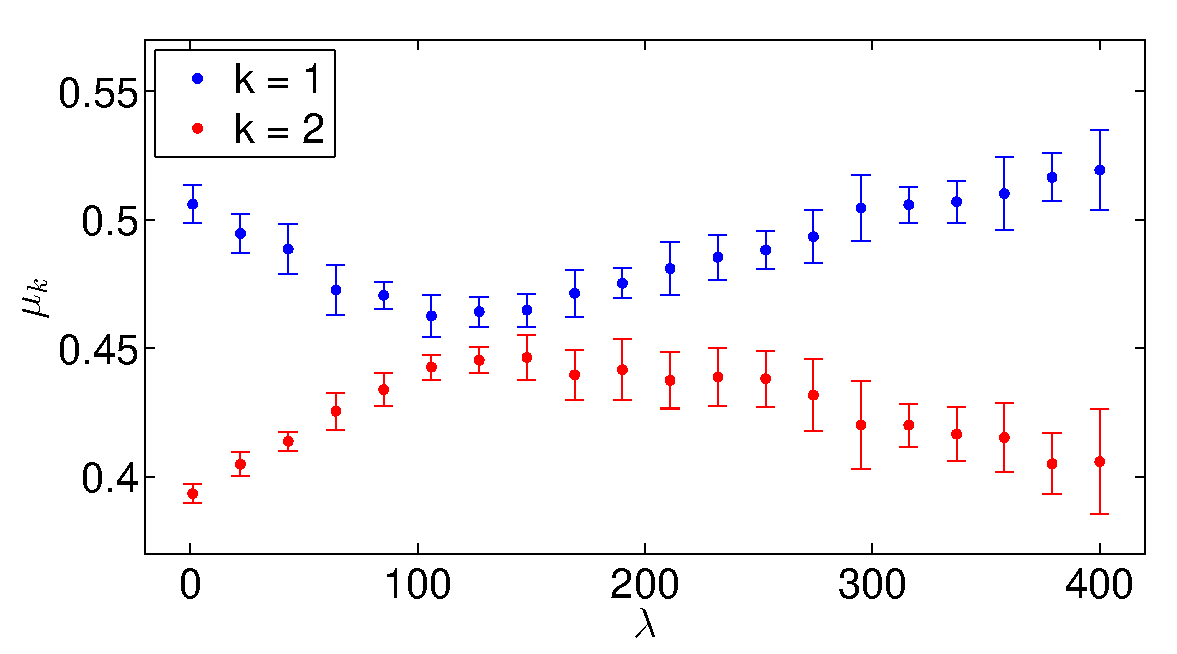
\includegraphics[width=0.5\textwidth]{detect_change_eigenvalues}
\caption{The first two eigenvalues from diffusion maps as a function of $\lambda$. Each point is averaged over $10$ simulation experiments (as in Figure~\ref{fig:dmaps_embed_emd}, one experiment consists of data collected at varying $p$ and $t$, for a fixed value of $\lambda$), with error bars denoting one standard deviation. 
The convergence of the eigenvalues at $\lambda \approx 125$ indicates switching of the dynamical ``mode''.}
\label{fig:detect_change}
\end{figure}

We have seen that the eigenvalues $\mu_i$, which quantify the importance of each embedding coordinate, reveal the relative importance of the variables which govern the macroscopic dynamics.
%
We can also use these eigenvalues to detect changes in dynamical behavior.
%
We expect a gap between the two eigenvalues at the two asymptotic regimes ($\lambda \rightarrow 0$ and $\lambda \rightarrow \infty$), as one of the two macroscopic variables is significantly more important to the dynamical behavior.
%
For intermediate $\lambda$ values, we expect the gap between $|\mu_1|$ and $|\mu_2|$ to narrow, with the $\lambda$ value where $|\mu_1| \approx |\mu_2|$ corresponding to the transition between ``wave-like'' and ``heat-like'' behavior. 

To demonstrate this point, we performed a new set of experiments, where we simulated the velocity jump process system over a range of $\lambda$ values. 
% 
Figure~\ref{fig:detect_change} shows the first two diffusion maps eigenvalues, $\mu_1$ and $\mu_2$, computed from these simulations, as a function of $\lambda$.
%
For small $\lambda$ (the wave-equation regime, corresponding to Figures~\ref{subfig:small_lambda_p}~and~\ref{subfig:small_lambda_t}), the two eigenvalues are well-separated, as the first mode (which parameterizes $p$) is significantly more important than the second mode (which parameterizes $t$).
%
At intermediate $\lambda$ values, the eigenvalues come together as the system dynamics change and both $p$ and $t$ are of similar importance.
%
The eigenvalues then separate again at large $\lambda$ (the heat equation regime, corresponding to Figures~\ref{subfig:large_lambda_p}~and~\ref{subfig:large_lambda_t}), where the $t$ effects dominate the dynamics.
%
We can therefore detect changes in dynamical behavior using data-driven techniques, without any knowledge of the governing macroscopic model. 

%\begin{figure}[t]
%\def\figwidth{4.2cm}
%\begin{subfigure}{\figwidth}
%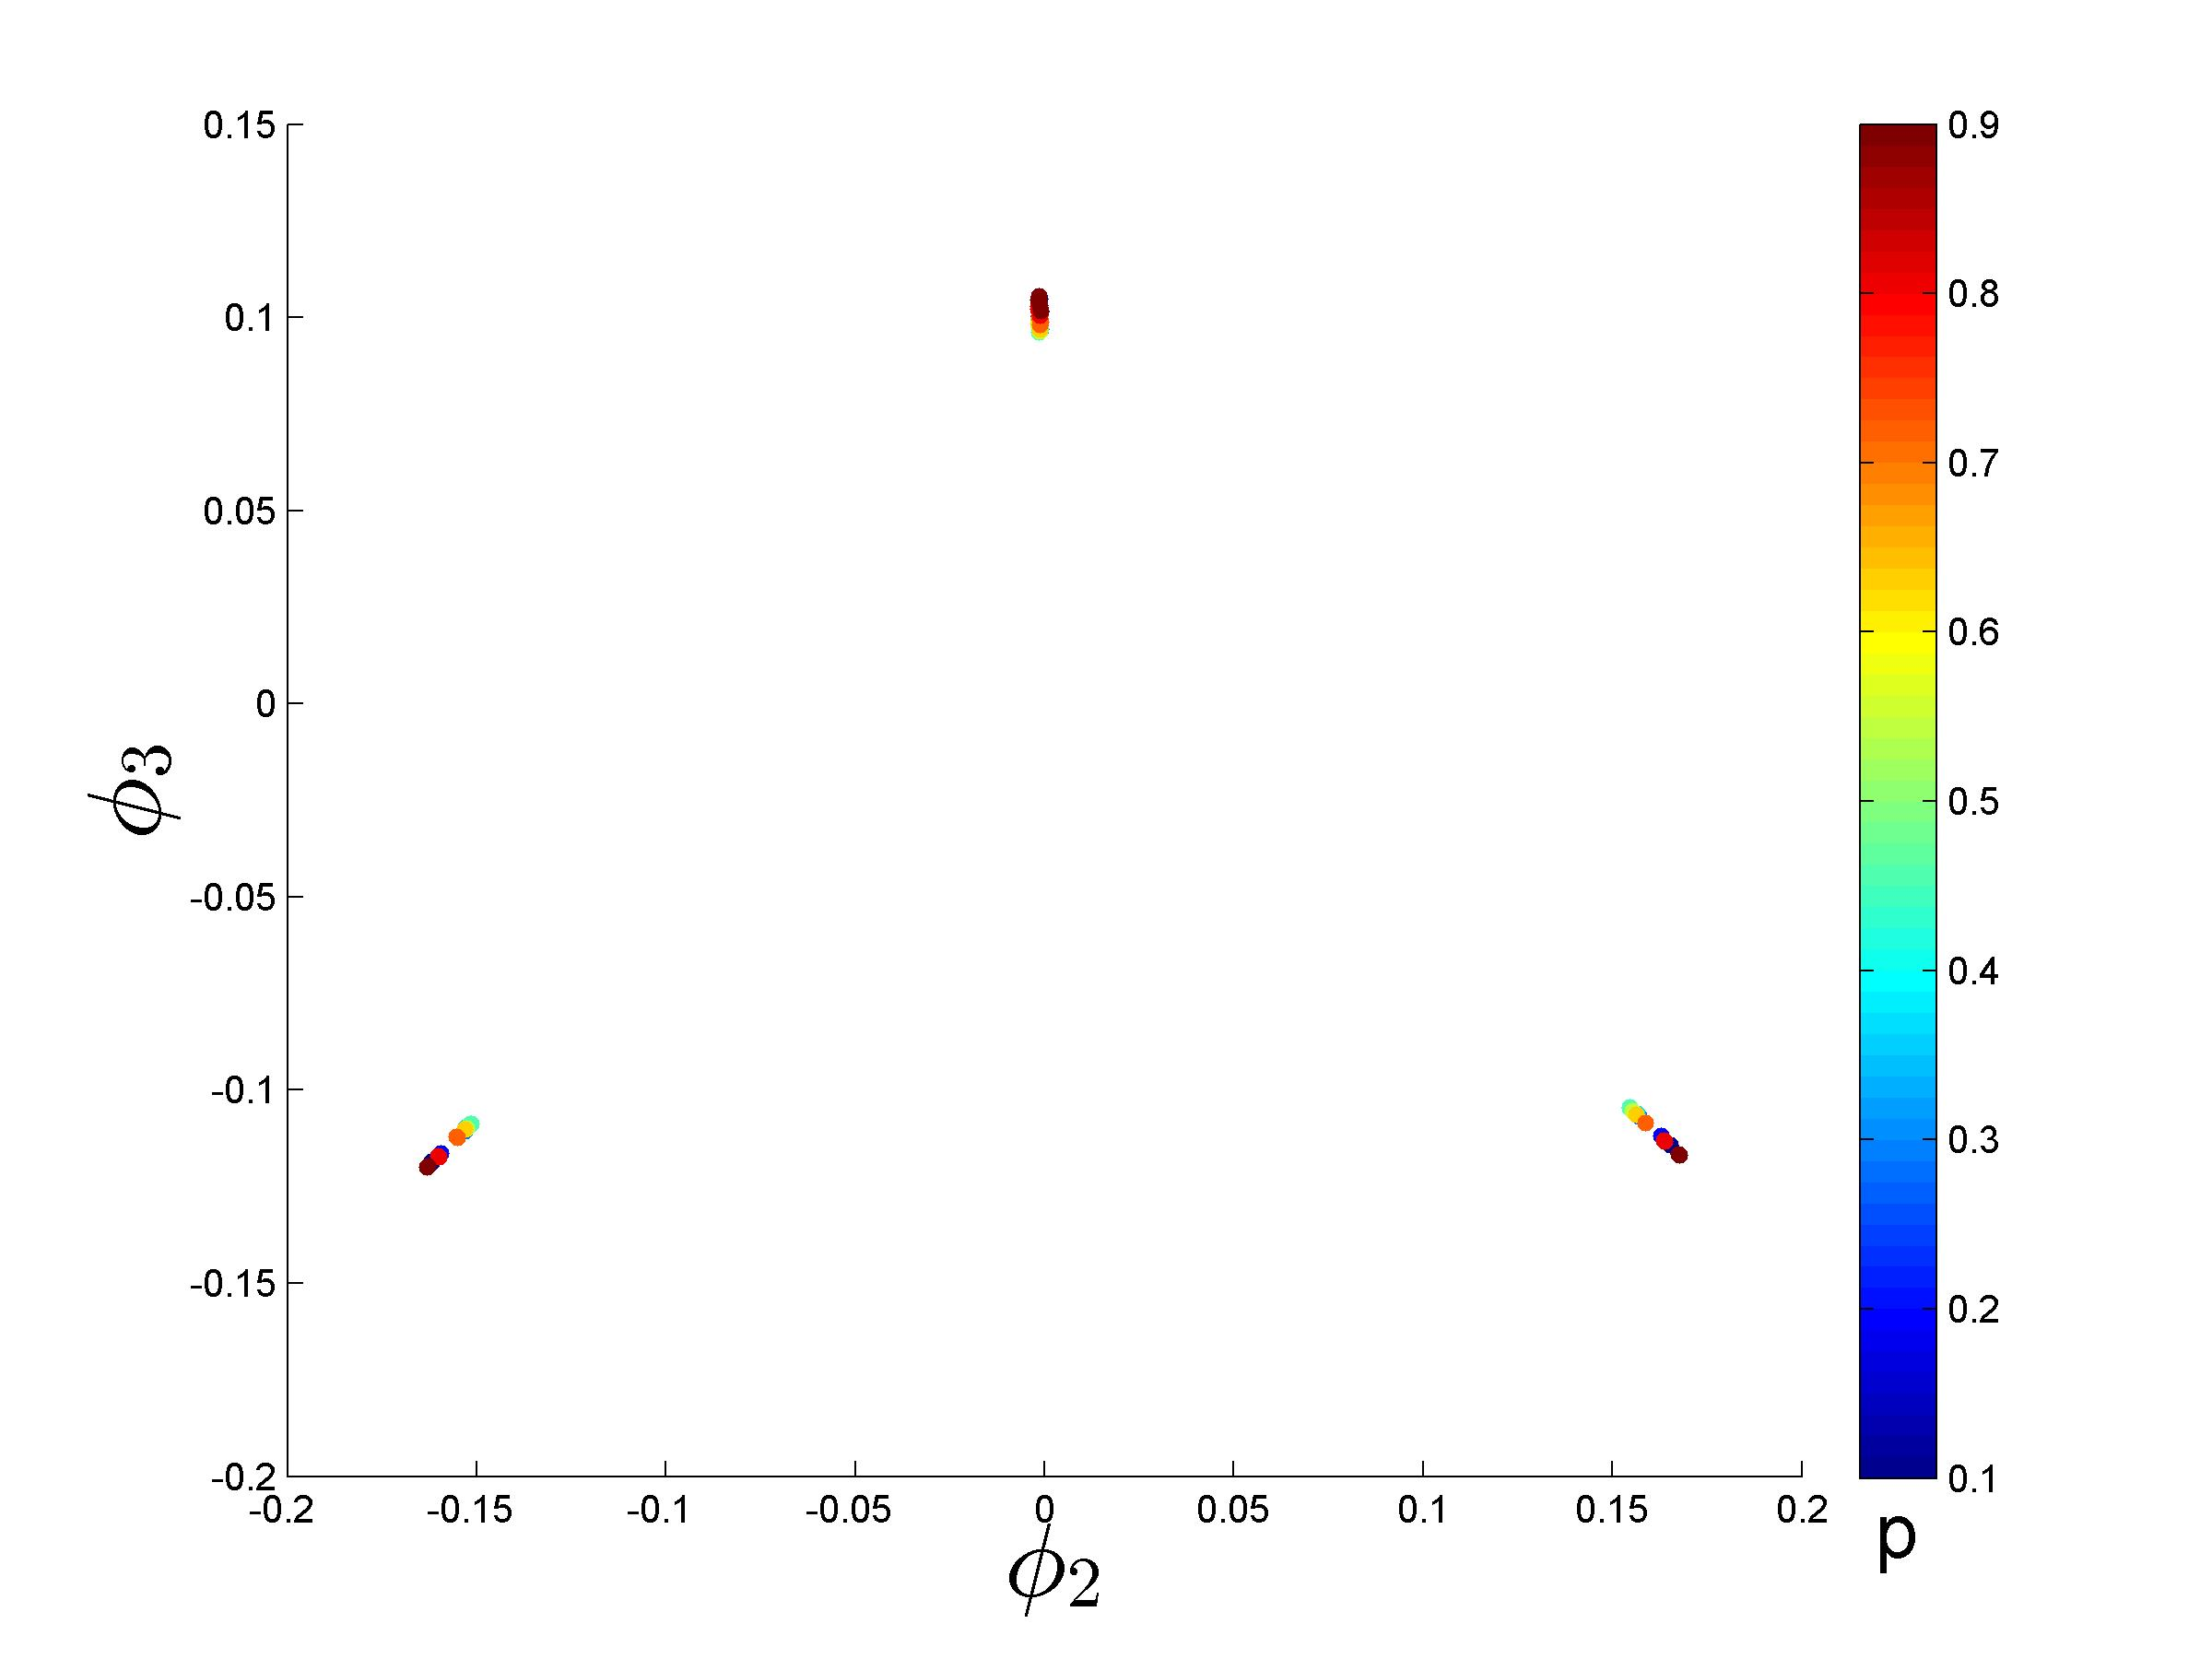
\includegraphics[width=\textwidth]{rawhist_p_1}
%\caption{}
%\end{subfigure}
%\begin{subfigure}{\figwidth}
%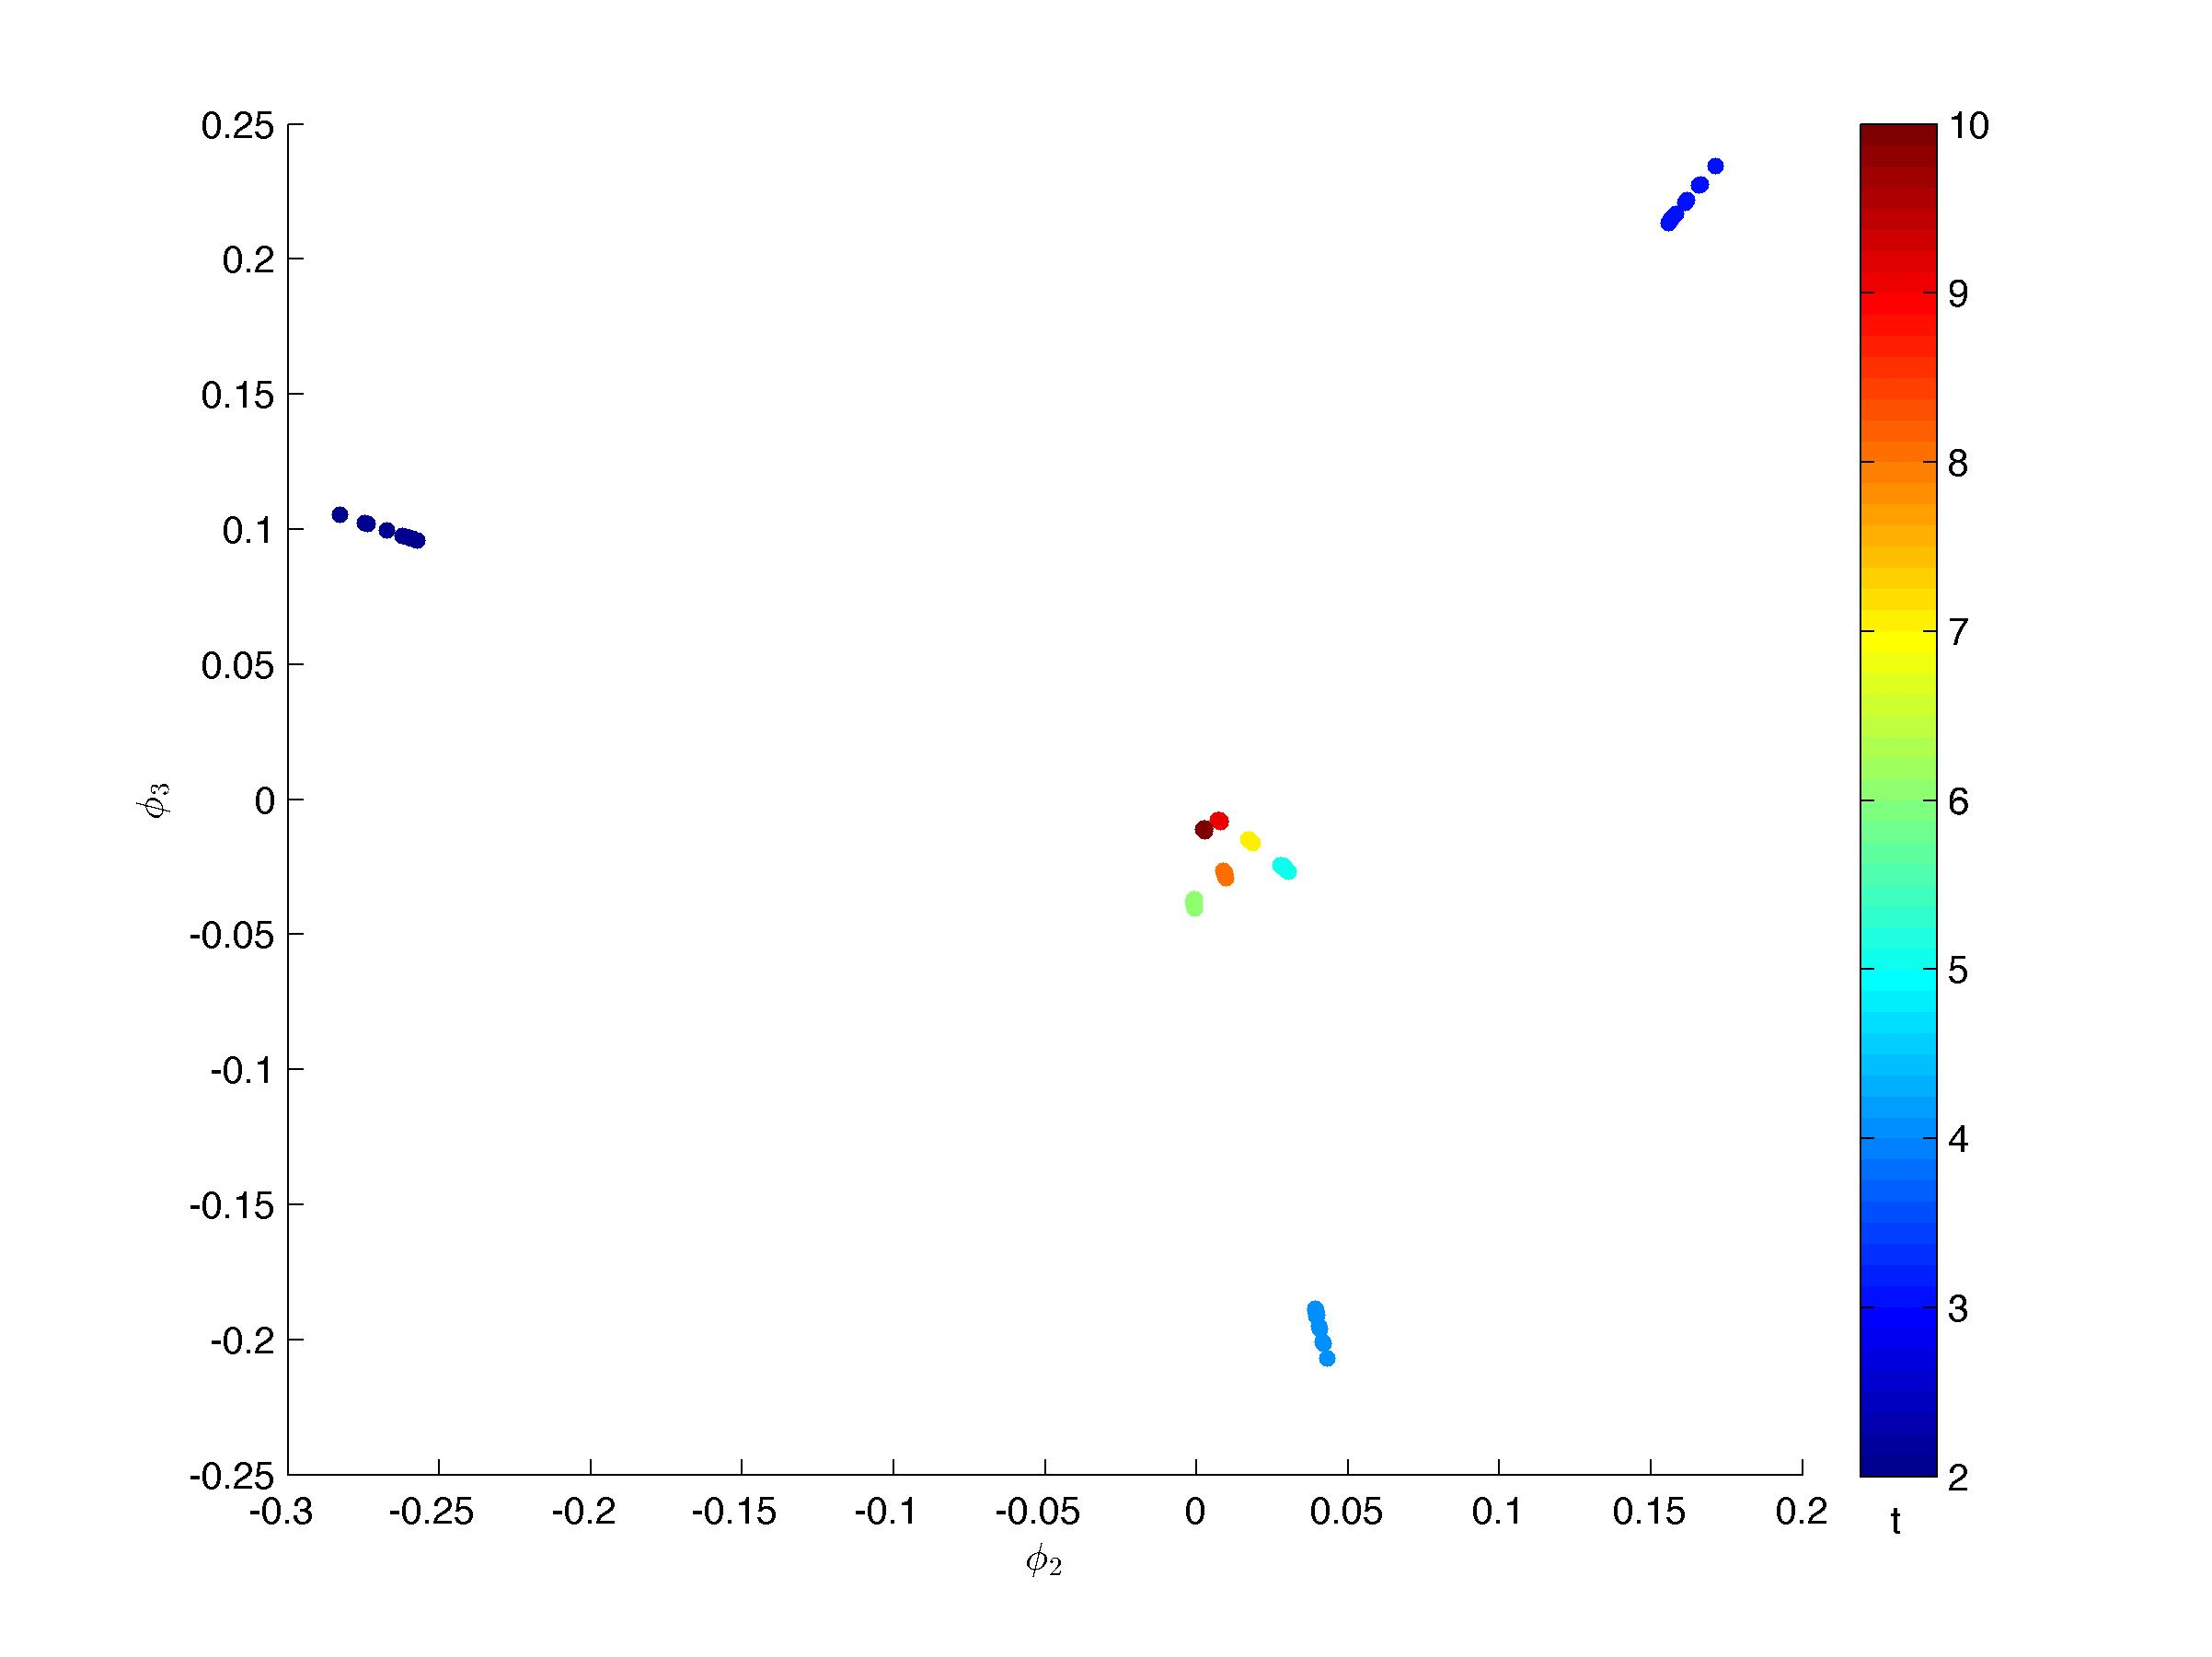
\includegraphics[width=\textwidth]{rawhist_t_1}
%\caption{}
%\end{subfigure}
%\begin{subfigure}{\figwidth}
%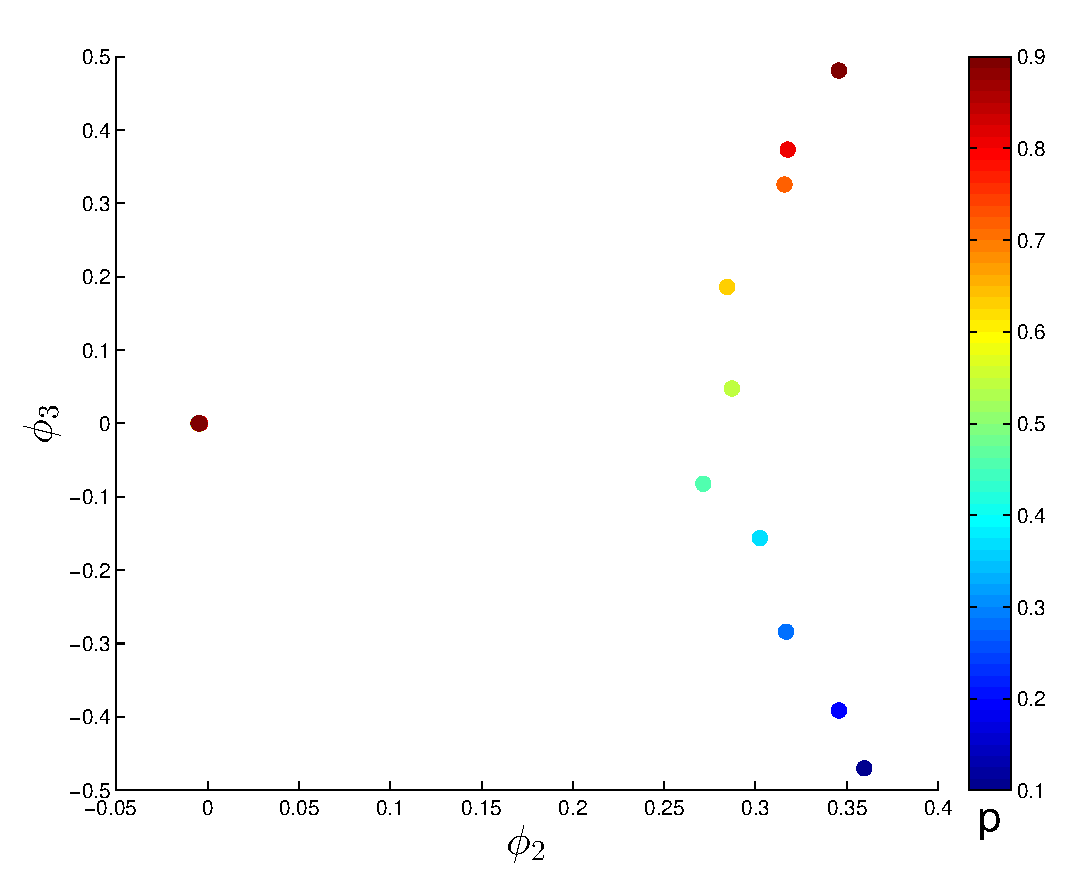
\includegraphics[width=\textwidth]{rawhist_p_400}
%\caption{}
%\end{subfigure}
%\begin{subfigure}{\figwidth}
%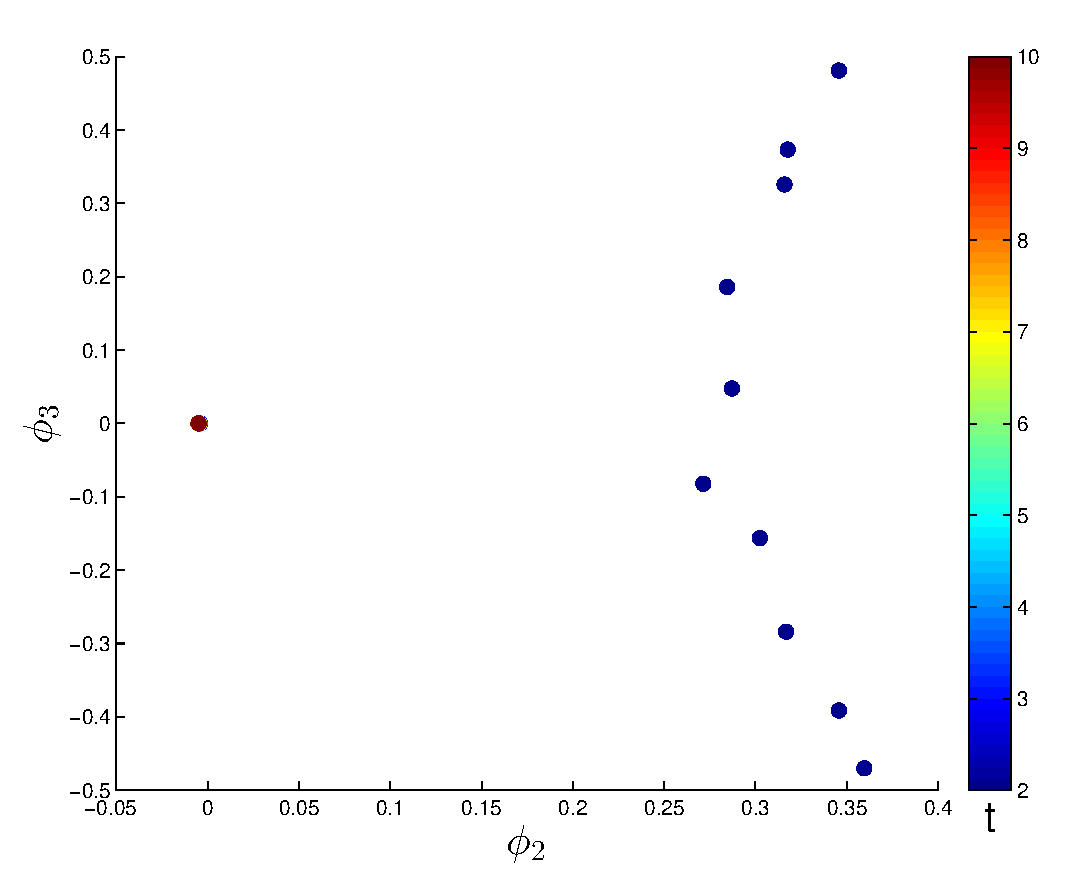
\includegraphics[width=\textwidth]{rawhist_t_400}
%\caption{}
%\end{subfigure}
%\caption{Diffusion maps embeddings computed from simulation data of the velocity jump process with (a,b) $\lambda=1$, $s=1$, and (c,d) $\lambda=400$, $s=20$. The distances used in the diffusion maps kernel are the Euclidean distances between the histograms of particle positions. The data are colored by (a, c) $p$, the initial probability of a particle moving to the right, and (b, d) $t$, time.}
%\label{fig:dmaps_embed_noemd}
%\end{figure}



\subsubsection{Detecting changes in dimensionality}

\begin{figure}
%
\def\figheight{1.4in}
%
\begin{subfigure}[t]{0.31\textwidth}
\centering
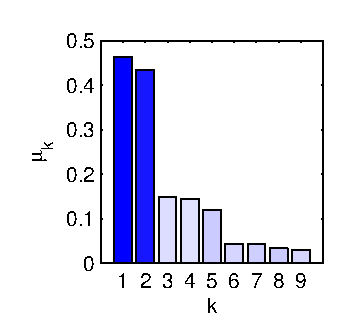
\includegraphics[height=\figheight]{chemotaxis1_evals}
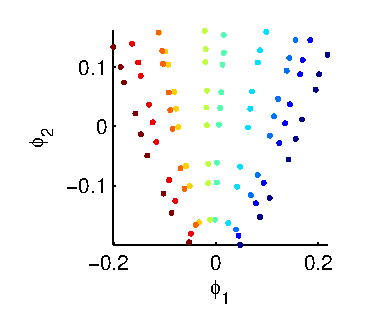
\includegraphics[height=\figheight]{chemotaxis1_embed_good}
\vspace{1.2in}
%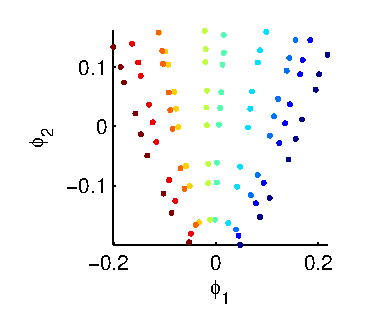
\includegraphics[height=1.5in]{chemotaxis1_embed_bad}
\caption{}
\end{subfigure}
%
\begin{subfigure}[t]{0.31\textwidth}
\centering
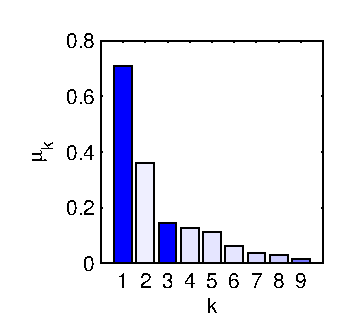
\includegraphics[height=\figheight]{chemotaxis2_evals}
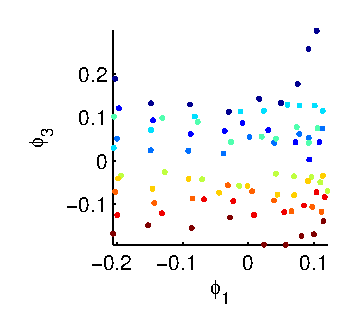
\includegraphics[height=\figheight]{chemotaxis2_embed_good}
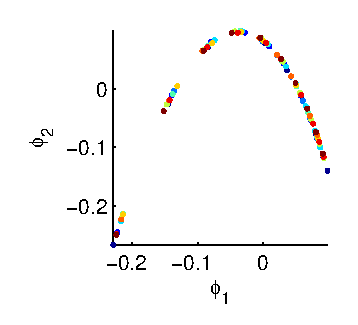
\includegraphics[height=\figheight]{chemotaxis2_embed_bad}
\caption{}
\end{subfigure}
%
\begin{subfigure}[t]{0.35\textwidth}
\centering
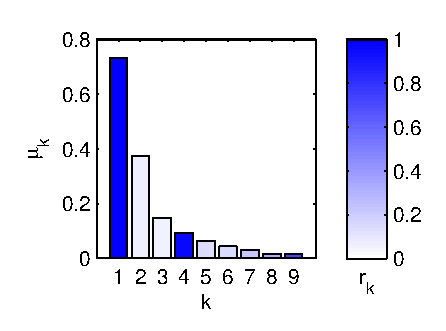
\includegraphics[height=\figheight]{chemotaxis3_evals}
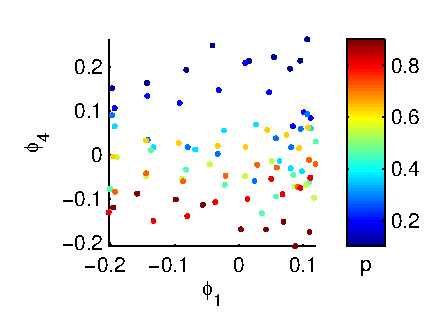
\includegraphics[height=\figheight]{chemotaxis3_embed_good}
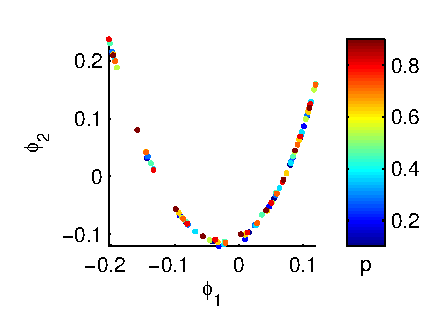
\includegraphics[height=\figheight]{chemotaxis3_embed_bad}
\caption{}
\end{subfigure}
%
\caption{Diffusion maps embedding for three different chemotaxis simulations. (a) $\lambda = 100$, $s = 10$. (b) $\lambda = 2500$, $s = 50$. (c) $\lambda = 6400$, $s = 80$. For each simulation, the eigenvalue spectrum is shown. From the spectra, we can see that the first two components are informative for (a), components 1 and 3 are informative for (b), and components 1 and  are informative for (c). The corresponding embeddings are shown below. For comparison, the embeddings using the first two components are also shown in (b) and (c), where clearly, the second component is a harmonic of the first and does not describe a new direction in the data. }
%
\label{fig:chemotaxis_simulations_harmonics}
\end{figure}

\begin{figure}[t]
%
\centering
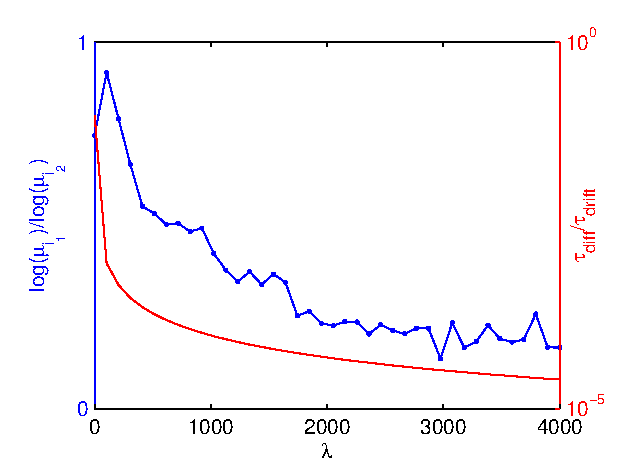
\includegraphics[width=0.5\textwidth]{chemotaxis_compare_timescales_evals}
%
\caption{Detecting the change in dimensionality. The ratio of the log of the two ``meaningful'' diffusion maps eigenvalues (those which correspond to modes which are not harmonics) is shown in blue, and the ratio of the diffusive and drift time scales are shown in red. When the diffusive time scale is significantly larger than the drift time scale, the data is expected to be effectively one-dimensional. This transition is consistent with the diffusion maps eigenvalues: the data is effectively one-dimensional if the first eigenvalue is significantly larger than the second. }
%
\label{fig:chemotaxis_compare_timescales_evals}
%
\end{figure}

Often in dynamical systems, one would like to detect a change in the dimensionally of the system. 
%
We can uncover the true dimensionally of the data set by looking at the eigenvalues corresponding to eigenvectors which parameterize new directions in the data. 
%
For the specific chemotaxis example, we know that there are two directions in the data, corresponding to simulation parameters $p$ and $t$. 
%
However, for large values of $\lambda$, we know the dynamics become diffusive and $p$ becomes unimportant; we therefore expect the data to look approximately one-dimensional when $\lambda$ is large. 

To detect this transition in the data, we look at the eigenvalues corresponding to the two independent eigenevctors. 
%
Let $\mu_{i_1} \ge \mu_{i_2}$ denote these two eigenvalues. 
%
According to \eqref{eq:est_lengths}, we plot  
\begin{equation}
 \sqrt{\frac{\log \mu_{i_1}}{\log \mu_{i_2}}} ;
\end{equation}
when this ratio becomes small, the data are effectively one-dimensional, as the second dimension is very small compared with the first. 
%
Figure~\ref{fig:chemotaxis_simulations_harmonics} shows the eigenvalue spectra for three different sets of simulations. 
%
It now becomes clear that looking at the diffusion maps coordinates {\em modulo} higher harmonics is essential for extracting an informative parameterization of the data, as well as characterizing the dimensionality of the data. 
%
From Figures~\ref{fig:chemotaxis_simulations_harmonics}(b-c), we can see that the eigenvalue spectrum does not exhibit any large spectral gaps.
%
However, there is a significant gap between the eigenvalues which correspond to new directions in the data, and the corresponding eigenvectors provide us with a two-dimensional parameterization of the data which is consistent with the expected macroscopic dynamics. 



Figure~\ref{fig:chemotaxis_compare_timescales_evals} shows the diffusion maps eigenvalue ratio as a function of $\lambda$. 
%
For this specific example, we can compare the empirically detected change in dimensionality with the analytically-predicted shift. 
%
From \cite{othmer2000diffusion}, the relevant time scales for the velocity jump process are
%\begin{equation}
%\begin{aligned}
%\tau_{drift} =& \frac{L}{s} \\
%\tau_{diff} =& \frac{L^2 \lambda}{s^2}
%\end{aligned}
%\end{equation}
%%
%Here, we take $L = t_{max} s$ as a characteristic length scale for the simulations. 
%
\begin{equation}
\begin{aligned}
\tau_{drift} =& t_{max} \\
\tau_{diff} =& t_{max}^2 \lambda
\end{aligned}
\end{equation}
%
When $\frac{\tau_{diff}}{\tau_{drift}} =  t_{max}  \lambda \gg 1$, then the dynamics are effectively one-dimensional. 
%
This ratio is also plotted in Figure~\ref{fig:chemotaxis_compare_timescales_evals} as a function of $\lambda$, and the transition is consistent with the transition predicted by the diffusion maps eigenvalues. 



\section{Conclusions}

This paper aims to bridge the fields of data mining and dynamical systems. 
%
For data mining methods to be informative with regards to the underlying system dynamics, processing the appropriate statistical moments or observables instead of individual particles is essential. 
%
In addition, one must also define the appropriate distance metric between the observations.
%
These two components induce the ``correct" Riemannian geometry and allow for informative analyses, such as meaningful and compact parameterization, phase shift detection, and dynamical characterization, through manifold learning.
%
In this paper, these concepts were demonstrated using a dynamical model of cellular chemotaxis with a known macroscopic behavior.
%
We showed that, using histograms as observers and EMD as a distance metric, diffusion maps can uncover a parameterization of the microscale data which is consistent with the analytic macroscopic model.
%
We are confident that such techniques can help inform modeling efforts for systems where the macroscopic dynamics and behavior are not currently known. 


\section*{Acknowledgment}
The authors would like to thank TODO.

\bibliographystyle{elsarticle-num}
\bibliography{../../../references/references}

\end{document}
